%
% Modified Monday, 26 September
%

\newcommand{\akcomment}[1]{
\textcolor{olive}{\textbf{AK: }\footnotesize #1}}

\newcommand{\khcomment}[1]{
\textcolor{magenta}{\textbf{KH: }\footnotesize #1}}

\newcommand{\fixlink}[1]{\textcolor{red}{Fix link!}}

\newcommand{\khaction}[1]{
\textcolor{red}{\textbf{Action: }} #1
}

\section{Overview of the department and its context}
\label{sec:overview}



% \akcomment{1. focus on providing the information specifically requested in each 
% question. Some discussion relates more to other questions (including, e.g, s 
% 1.2.1, 1.3.b).  Eliminate information that doesn't clearly relate to the 
% question.
% }

% \akcomment{
% The assessment criterion for Section 2 is "evidence-based recognition of the 
% issues and opportunities facing the applicant." To meet this criterion, focus 
% the narrative in each sub/section by saying explicitly what the data in each 
% section reveals about the gender equality challenges (or 
% strengths/opportunities) the School faces - spell this out for the reviewer.  
% The key function of section 2 is to 'diagnose' key attrition points in the 
% pipeline (from UG through Prof), and also to identify which 3 - 5 of these key 
% challenges the School will attempt to address in the action plan.  While it's 
% useful (p.20) to cite to actions from later in the application that will begin 
% to address these key challenges, you are not expected to flesh out these actions 
% in Section 2.  Thus, e.g, Actions 2.1.2 and 2.1.3 (p. 20) might sit better in 
% section 2.1.e, where there might be opportunity to clarify the rationale for 
% these actions.
% }

% The School comprises around 80 staff across all categories and grades
% as well as close to 700 students ranging from undergraduates to PhD 
% students These numbers include those belonging to a number of large 
% research groups/centres in the school.
% This includes Insight whose research focus is on constraints,
% AI and data analytics
% and also includes Connect devoted to research broadly
% on networks and communication technologies. 
% These two centres account for a significant 
% proportion of the school's research students and staff.



\subsection{Provide a description of the department’s structures to advance equality. This should include:}  
\instr{
\begin{itemize}
\item teaching and research focus, including discipline coverage and any areas of specialism;
\item	the total number of staff by gender and category of post; 
\item	the total number of students by programme type and gender;
\item	information on location/s.
\end{itemize}
}

\subsubsection{Teaching and research focus}

% \khcomment{Programme-summary table moved to student-numbers section.
% Replace with table with brief description of school's main 
% offerings. Rip this from old Quality Review document from 2018.
% Include year of introduction info.
% }


Table~\ref{tab:teachingoverview} presents an overview of the school's
main teaching activities. 
%The portfolio includes three programmes focused on core computer science (BSc, MSc and a Higher Diploma conversion course).
The school has strategically diversified its portfolio in the
last decade by introducing a suite of interdisciplinary programmes
(denoted \interdis)
in Data Science (BSc and MSc), Digital Humanities (BA), Interactive 
Media (MSc) and Psychology and Computing (BA). This 
diversification was designed to increase student  numbers overall and  
especially to improve the gender balance in our student body. 
%The impact of these initiatives on gender balance is explored further in Subsection~\ref{sec:ug_data}.
The school also contributes significantly to other programmes  within 
the university through service teaching to Arts, Science, and 
Engineering students at both undergraduate and postgraduate level.

\input{tables2/tab_teaching_focus_new}


% \akcomment{Table 2.3 (nice table): include PGR student data.   Add totals for 
% UG, PGT, PGR students.  Match the table header to the application question 
% (i.e. change Table 2.3. header from "Overview of School's Taught Programmes" to 
% "Total number of students by programme type and gender".}

% \akcomment{
% On page 20, an explanation is given that the School diversified degree 
% programmes "to increase student numbers overall and especially to improve the 
% gender balance in our student body". This seems both interesting and important.  
% Can more be said about this?   E.g. which programmes? Is the impact of this 
% effort reflected in the data presented in this section? (How/not?)    Similarly, 
% mention is made of CRTs' "specific remit to consider gender equality in 
% recruitment" - is the impact of this evident in the data presented in this 
% section? How/not?
% }

Research in the school is clustered into four thematic areas:
\begin{enumerate}[noitemsep]
    \item Artificial Intelligence, Data Analytics and Algorithmics
    \item Networks, Computer Architectures and Software Systems 
    \item Interactive Media and Human Computer Interaction
    \item Security, Privacy and Ethics
\end{enumerate}

% \khcomment{Add para on research strengths. 
% Thumbnail sketch (one para, 4-5 lines) of Insight and Connect.}

Much of this research is conducted within a number of funded research groups and centres (see 
Table~\ref{tab:researchcentres}), as well as two centres for research training (CRTs) (see Table~\ref{tab:crts}) that are hosted within the school. Both CRTs have an explicit gender quota for enrolment. 
%Gender issues relating to PhD students are analysed in Subsection~\ref{sub:phdnumbers}.
%summarises the main funded research groups and centres within the school.

\begin{tabbox}{!t}

\caption{Funded research centres within or affiliated with the school}
\label{tab:researchcentres}
\footnotesize 

\sisetup{
    group-digits=all,
    group-minimum-digits=4,
    mode=text,
    reset-text-series = false, 
    text-series-to-math = true,
    reset-text-family=false, 
    text-family-to-math=true
}
% 'preamble ends here'

\begin{tabular}{p{2.5cm}
                p{7.5cm}
                !{\qquad}
                p{4cm}
                }
\toprule 
Name & Focus & Website\\ 

\midrule 

Insight&
Data science, analytics, and artificial intelligence, including decision optimisation & \url{https://www.insight-centre.ie}\\
\hdashline
Connect&
Future networks and communications & \url{https://connectcentre.ie/}\\
\hdashline
Enable&
Smart environments & \url{https://www.enable-research.ie/}\\
\hdashline
Confirm&
Smart manufacturing & \url{https://confirm.ie/} \\
\hdashline
Lero&
Software research, including complex
systems & \url{https://www.lero.ie}\\
\hdashline
MISL&
Networks and systems, with a focus on mobile/wireless and multimedia & \url{https://www.ucc.ie/en/misl/}\\

\bottomrule 
\end{tabular}

\end{tabbox}




\begin{tabbox}{!t}

\caption[Centres for research training in the school]{Centres for research training (CRTs) in the school}
\label{tab:crts}
\footnotesize 

\sisetup{
    group-digits=all,
    group-minimum-digits=4,
    mode=text,
    reset-text-series = false, 
    text-series-to-math = true,
    reset-text-family=false, 
    text-family-to-math=true
}
\begin{tabular}{p{2.5cm}
                p{7.5cm}
                !{\qquad}
                p{4cm}
                }
\toprule
Name & Focus & Website\\ 
\midrule 

%  Lifted from 2018 Quality Review report
% Originally established by Prof. Eugene Freuder (Emeritus) as the Cork
% Constraint Computation Centre in 2001, rebranded in 2013 to Insight, the 
% SFI-funded Research Centre for data science
% & analytics, including decision optimisation. 
% Partner in the SFI-funded Confirm Research Centre for smart
% manufacturing and SFI-funded ENABLE research programme for smart
% environments. 

% Lifted from 2018 Quality Review report
% MISL (Mobile & Internet Systems Lab)
% Computer networking, especially wireless.
% Partner in the Connect SFI-funded
% Research Centre for future networks and
% the SFI-funded ENABLE research
% programme for smart environments



CRT-AI&
SFI programme to provide research training
in Artifical Intelligence;
Provides funding for 120 PhD students over four
years between 2019-2023 across five partner 
institutions. & \url{https://www.crt-ai.ie/} \\
\hdashline
Advance-CRT&
SFI programme to provide research training
on future networks and the Internet of Things with
applications for sustainable and independent living;
Provides funding for 120 PhD students over four
years between 2019-2023 across five partner 
institutions. & \url{https://www.advance-crt.ie/} \\

% Material from here on copied verbatim from model.
\bottomrule 
\end{tabular}


\end{tabbox}




%As shown in Table~\ref{tab:crts} the school hosts two centres for research training (CRTs): CRT-AI (Artificial Intelligence) hosted within Insight and ADVANCE-CRT (Advanced Networks for Sustainable Societies). These have an explicit  gender quotas for enrolment. Gender issues relating to PhD students are analysed in Subsection~\ref{sub:phdnumbers}, including the impact of the introduction these two centres.



\subsubsection{Staff count by gender and category of post}

Table~\ref{tab:headcount} provides an overview of the numbers of staff in the school per 2020. 
Professional, Managerial, and Support Staff (PMSS) includes 
both those in administrative roles and in IT support roles.  
%While this snapshot  relates to 2020, the salient features have 
%not shifted materially since. 
%Student numbers are included to
%give a sense of scale.
%
\input{tables2/tab_headcount}
%
%A more detailed exploration of the gender balance across categories appears later (Subsection~\ref{sec:academic_research} for academic and research staff, Subsection~\ref{sec:pms} for PMS staff), but it 
It is evident 
that females are under-represented in almost all categories, most 
starkly among research and  academic roles. The school is acutely 
aware of this imbalance  and it is a strategic priority for the 
school to address this over time.

Table~\ref{tab:keyroles} summarises leadership roles
within the school, which clearly shows a significant under-representation of females, reflecting a dearth of women in senior grades across all staff categories. 
The term ``Director'' in Table~\ref{tab:keyroles} refers to senior
director-level leadership roles in one of the multi-institutional 
SFI-funded national research centres that the school is involved in (see Table~\ref{tab:researchcentres}) as well as the two SFI-funded centres for training PhD students (see Table~\ref{tab:crts}). 
Since their inception in 2019, these CRTs have provided a 
significant proportion of the PhD students in the school.


\begin{tabbox}{!th}

\caption{Key roles within CSIT by gender}
\label{tab:keyroles}
\footnotesize 

\sisetup{
    group-digits=all,
    group-minimum-digits=4,
    table-format=2.1,
    mode=text,
    reset-text-series = false, 
    text-series-to-math = true,
    reset-text-family=false, 
    text-family-to-math=true
}
\begin{tabular}{p{4cm}
                S[table-format=2.1]
                !{\quad}
                S[table-format=2.1] 
                p{3cm} 
                p{4cm} 
                S[table-format=2.1]
                !{\quad}
                S[table-format=2.0] 
                }
\toprule 
\multicolumn{3}{c}{\textmd{School Leadership}} %JPM Changed Academic to School
&&
\multicolumn{3}{c}{\textmd{Research Leadership}}\\ 
\cmidrule{1-3}\cmidrule{5-7}
& {F} & {M} & & & {F} & {M} \\ 
\midrule 
Head  of School  & 0 & 1 && Research Directors\interdis & 0 & 4\\ %JPM Changed Directors to Research Directors
\cdashline{1-3}\cdashline{5-7}
PMS Managers & 1 & 1& & Principal Investigators & 0& 10\\
\cdashline{1-3}\cdashline{5-7}
%AOD, GP, GR, IP, AZ, MvD, KJS, DM
Programme Directors & 2 & 6 & & SFI Funded Investigators\interdis\interdis & 1& 8\\
\cdashline{1-3}
Committee Chairs& 0 & 8 &&&&\\
\bottomrule 
\end{tabular}
\begingroup
\sffamily 
\singlespacing 
\interdis{} Director refers to Directors or Co-Directors of SFI Research Centres.\\
\interdis\interdis{} SFI Funded Investigator (FI) is a role within an SFI Research Centre, such as Connect and Lero; an FI leads one or more research projects within such a centre, and must be approved by SFI.
\endgroup 

\end{tabbox}


\subsubsection{Student count by programme type and gender}

%A summary of student numbers acroos the various programmes in the school's teaching portfolio  by programme and gender appears in 
Table~\ref{tab:teachingportfolio} summarises student numbers and female participation within the school. 
%
% \khcomment{Add caption: ``Total number of students by programme type
% and gender.''; Fill in the missing totals, as follows: UG (total 511,
% percentage 24\%; PGT (total 129, percentage 46\%; PGR (total 43,
% percentage 12\%)
% }
%
The flagship course BSc in Computer Science programme,
similar to most CS programmes in Europe and North America,
has always struggled with under-representation of females. 
%Within the last decade the School introduced a number of interdisciplinary programmes  (marked with \interdis) to improve gender equality in the composition of its undergraduate student body. 
The table also includes numbers
of PhD students for 2020. PhD numbers have climbed steadily 
in recent years as has the gender balance of those enrolled.
%This issue is explored further in  Subsection~\ref{sec:phdnumbers}.


\begin{tabbox}{!th}

\caption[Number of students by programme and gender]{Number of students by programme and gender (2020)}
\label{tab:teachingportfolio}
\footnotesize 

\sisetup{
    group-digits=all,
    group-minimum-digits=4,
    mode=text,
    reset-text-series = false, 
    text-series-to-math = true,
    reset-text-family=false, 
    text-family-to-math=true
}
\begin{tabular}{P{3.5cm}
                !{\qquad}    
                p{7cm}
                S[table-format=3.0]
                !{\quad}
                S[table-format=2.0\%] 
                %C{3cm}
                }
\toprule 

& \textmd{Programme}&  {\textmd{\makecell{Student count\\ (2019-20)}}} & {\textmd{\makecell{Female \\ \%} }} \\ 
\midrule
\multirow{2}{=}{Undergraduate programmes} & 
BSc in Computer Science& 286 & 14\%\\ 
\cdashline{2-4}
&BA in Digital Humanities and IT\interdis& 120 & 44\%\\ 
\cdashline{2-4}
&BSc in Data Science and Analytics\interdis&  51 & 20\% \\
\cdashline{2-4}
&BA in Psychology and Computing\interdis& 54 & 39\% \\
\cdashline{2-4}
&Subtotal undergraduate students & 511 & 24\% \\ 

\midrule 
\multirow{2}{=}{Postgraduate taught programmes} 
& Higher Diploma  in Applied Computing&22 & 41\% \\ 
\cdashline{2-4}
& MSc in Interactive Media&38 & 68\%\\ 
 \cdashline{2-4}
& MSc in Computing Science&30 & 33\%\\
 \cdashline{2-4}
& MSc in Data Science and Analytics\interdis&39 & 36\%\\
 \cdashline{2-4}
& Subtotal postgraduate students &129 & 46\% \\ 
 
\midrule 
Postgraduate research
& 
PhD students & 43 & 12\% \\ 

\bottomrule 
\end{tabular}

\end{tabbox}


% \khcomment{Include to indicate trajectory is upwards.}
% 

\subsubsection{Locations}
The School is housed in a single location in the Western Gateway 
Building (WGB) on campus (see Figure~\ref{fig:wgb}) which hosts virtually 
all of its teaching and research activity. On occasion, some lectures are scheduled in Brookfield Health Sciences Complex, which is located next to the WGB.

\begin{SCfigure}[10][!ht]
\hspace{-3pt}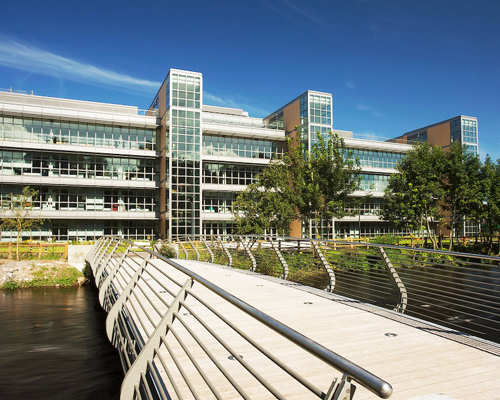
\includegraphics[width=3in]{img/WGB.jpg}
\caption{Western Gateway Building: home to CSIT}
\label{fig:wgb}
\end{SCfigure}


\newpage 
\subsection{Analyse three years of data on undergraduate students by}
\label{sec:ug_data}
\instr{
\begin{itemize}
\item gender and degree programme, with reference to discipline-specific benchmark data; 
\item gender and degree attainment;
\item gender and foundation courses.  
\end{itemize}
}

\subsubsection{Three years of data on undergraduate students by gender and degree programme}

Figure~\ref{fig:ug:enrolment} summarises enrolment statistics for our
four undergraduate degree programmes listed in Table~\ref{tab:teachingportfolio}
for the three-year period
up to academic year 2019-20 with the gender breakdown for each.\footnote{Both the BSc in Data Science and Analytics and the BA in Psychology and 
Computing started  in 2018-19  and so there are no data for
2017-18.} The gender balance is markedly better for the interdisciplinary 
programmes, especially the two BA programmes.  



\begin{figbox}
    \caption{Enrolment undergraduate students 2017-2020}
    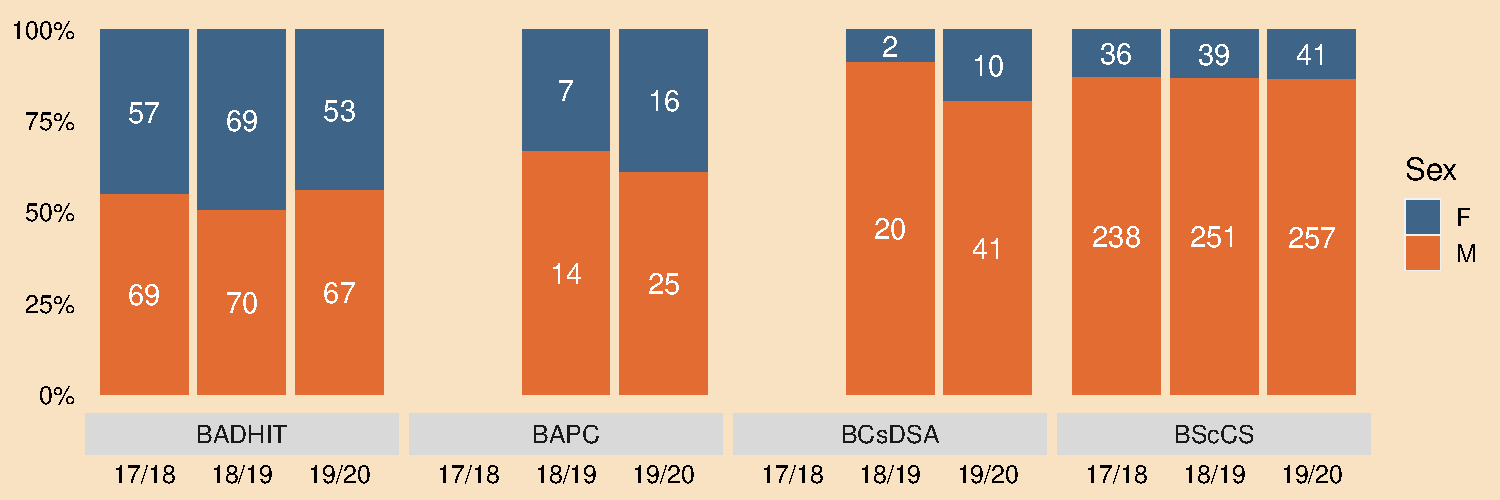
\includegraphics[width=\textwidth]{fig/ug_enrolment2.pdf}
    \label{fig:ug:enrolment}
\end{figbox}


Figure~\ref{fig:ug:mfintake} shows the evolution of the gender
breakdown linked to the introduction of new programmes
(BScDSA, BADHIT, BAPC). The more positive gender balance among 
newer programmes observed in Figure~\ref{fig:ug:enrolment}
has nudged the aggregate in a positive direction without
affecting the female participation rate for the BSc in Computer 
Science. 
The percentage of females overall improved slightly
from 24\% in 2017-18 to 25\% in 2021-22. 
%By way of comparison for 2009-10 (prior to the introduction of these newer programmes), the percentage of females was 14\%.


\begin{figure}[!ht]
\colorbox{orangebg}{
\begin{minipage}{14.2cm}
    \caption{Evolution of male/female intake for the BSc. CS programme vs. other undergraduate programmes within CSIT}
    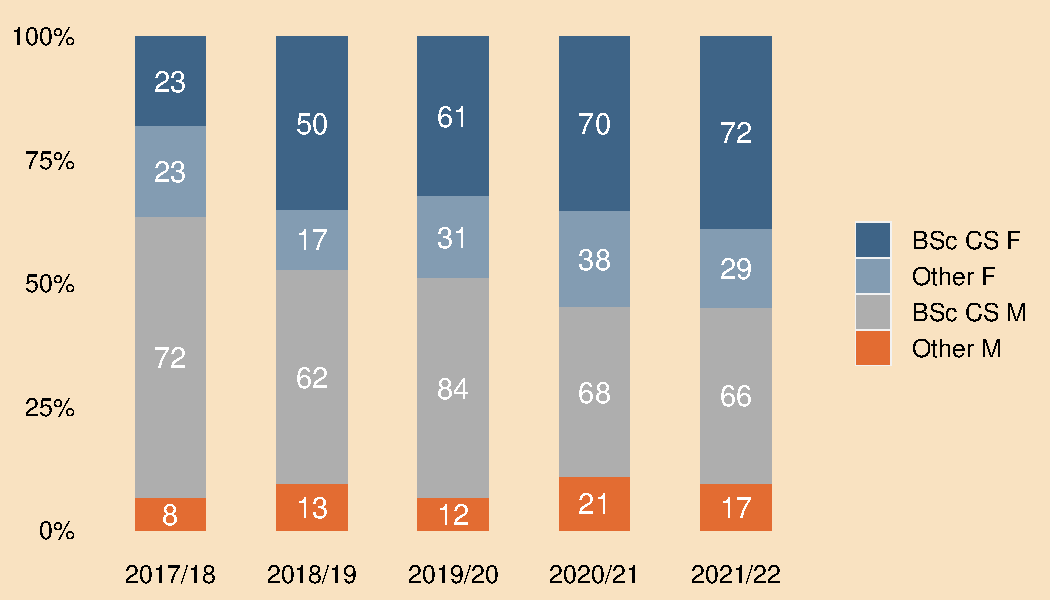
\includegraphics[width=5in]{fig/mfintake.pdf}
    
    \label{fig:ug:mfintake}
    \end{minipage}
}
\end{figure}

% \akcomment{Section 2.1.b: summarize detail on HESA/HEA benchmark data sources. I 
% find Fig. 2.3 confusing, esp. the inclusion of 2009/10 data (which raises new 
% questions in my mind).
% }

% \khcomment{Remove 2009-10 bar. Can we get pre-2014 enrolment and gender
% data for BScCS for comparison? Consider replacing figure with one with 
% two bars per year: one for BScCS and one for all programmes taken
% together. This might be less confusing?
% }

Table~\ref{tab:benchmarking:ug} compares CSIT's gender participation
rates for undergraduate taught programmes compared
with other institutions both in Ireland (HEA) and the UK (HESA).
Our female participation rates have improved over the period 
from 22\% to 24\%
and compare favourably with  Irish and UK benchmarks.  

% KH: Note sure we need quite so much detail here. Keep for now.
% KS: Moved to footnotes of table so it doesn't word-count.
% To compare the gender balance of CSIT programmes with HEA and 
% HESA data we note that:

% \begin{itemize}
%     \item The \ac{HEA} used the \ac{ISCED} and reports students studying \ac{ICT}, which covers ICT, Database and Network Design, and Software and Applications Development and Analysis. From 2019/2020 interdisciplinary programmes incorporating ICT are also included.
%     \item The UK \ac{HESA} \ac{HeCoS} aggregates the following subjects as Computing; computer science, information technology, information systems, software engineering, artificial intelligence, computer games and animation, business computing, and others in computing.
% \end{itemize}

From 2019/20 the HEA ICT grouping is in line with the combined programmes of CSIT. It is more difficult to compare the CSIT portfolio with the broader HESA HeCoS grouping as this incorporates information technology and information system programmes which have a wide variety of interpretations across the third level sector.

The F/M breakdown is approximately 19\% vs. 81\% across HEA ICT programmes 
across each of the years 2017/18 to 2019/20. The interdisciplinary programmes 
incorporating ICT have an approximately equal F/M breakdown in the years 2019/20 
and 2020/21.

% \khcomment{Compress. Suffices to say each benchmark is 
% based on different baskets of degrees/disciplines?}

\begin{table}[!htb]
\colorbox{SwanOrange!10}{
      \begin{minipage}{11.2cm}

\footnotesize       
\caption{Undergraduate male-female participation rates  benchmarked nationally
(HEA) and with the UK (HESA) (full-time students only)}
\label{tab:benchmarking:ug}
\sisetup{
    group-digits=all,
    group-separator = {,},
    group-minimum-digits=4,
    table-format=5.0,
    reset-text-series = false, 
    text-series-to-math = true
}
\begin{tabular}{p{2cm} 
                S[table-format=3.1]
                S[table-format=3.1]
                S[table-format=3.0\%]
                p{0.7cm}
                S[table-format=3.0]
                S[table-format=5.0]
                S[table-format=3.0\%]
                p{0.7cm}
                S[table-format=6.0]
                S[table-format=6.0]
                S[table-format=3.0\%]}
\toprule
  & \multicolumn{3}{c}{\textbf{UCC CSIT}} 
  &
  &\multicolumn{3}{c}{\textbf{HEA (Ireland)}} 
  &
  &\multicolumn{3}{c}{\textbf{HESA (UK)}}\\
  \cmidrule{2-4}\cmidrule{6-8}\cmidrule{10-12}
Year & {F}& {M} & {F\%} & & {F}& {M}& {F\%} & & {F} & {M} & {F\%}\\ 
 \midrule 
2017-18 & 95  & 344 & 22\% && 908 & 3762 & 19\% && 11080 &63250 &15\%\\
2018-19 & 117 & 355 & 25\% && 871 & 3664 & 19\% && 11965 &65935 &15\%\\
2019-20 & 121 & 390 & 24\% && 910 & 3755 & 20\% && 13635 &69800 &16\%\\ 
\bottomrule 
\end{tabular}
{
\sffamily

    The \ac{HEA} used the \ac{ISCED} and reports students studying \ac{ICT}, which covers ICT, Database and Network Design, and Software and Applications Development and Analysis. From 2019/2020 interdisciplinary programmes incorporating ICT are also included.
    The UK \ac{HESA} \ac{HeCoS} aggregates the following subjects as Computing; computer science, information technology, information systems, software engineering, artificial intelligence, computer games and animation, business computing, and others in computing.

}
\end{minipage}
}

\end{table}


CSIT's 22-24\% 
is somewhat better than the HEA figure of 19-20\% and 15-16\% for the 
UK/HESA. From Figure~\ref{fig:ug:enrolment} however
our undergraduate programmes exhibit wide variation in
female participation rates from 14-16\% in the BSc in Computer Science
to 44-50\% in BA in Digital Humanities, suggesting scope for improvement
in the former. As the  BSc in Computer Science aligns better
with the school's research programmes, any increase in female 
undergraduate numbers could over time provide a bigger pool 
of potential research postgraduates.


% \newcommand{\actdeptsurvey}{Survey current first year undergrads and taught postgrads on what influenced their course 
% choice, which recruitment initiatives are most effective and ideas for more balanced gender recruitment.}
% \begin{action}[label=action:dept:survey]{}
% \actdeptsurvey 
% \hfill{
%     \hypersetup{hidelinks}
%     \hyperlink{b0}{\gotoactionsymbol{}}
% }
% \end{action}

% \newcommand{\actdeptmarketing}{Review and amend marketing, advertising and recruitment strategy in light of data  
% received from surveys above.}
% \begin{action}[label=action:dept:marketing]{}
% \actdeptmarketing
% \hfill{
%     \hypersetup{hidelinks}
%     \hyperlink{b1}{\gotoactionsymbol{}}
% }
% \end{action}

% \newcommand{\actdeptrolemodels}{Actively boost visibility of female role models. Examples: video clips of recent grads 
% talking about their work; also interesting FYPs; also placements to illustrate range and diversity.}
% \begin{action}[label=action:dept:rolemodels]{}
% \actdeptrolemodels
% \hfill{
%     \hypersetup{hidelinks}
%     \hyperlink{b2}{\gotoactionsymbol{}}
% }
% \end{action}


% \newcommand{\actdeptfunds}{Expand prize and scholarship funds to better recognise student achievement.}
% \begin{action}[label=action:dept:funds]{}
% \actdeptfunds 
% \hfill{
%     \hypersetup{hidelinks}
%     \hyperlink{b3}{\gotoactionsymbol{}}
% }
% \end{action}

\subsubsection{Three years of data on undergraduate students by gender and 
degree attainment}

% \akcomment{Section 2.1.b - UG degree attainment.  The conclusion drawn from this 
% data is that "females are well represented among those receiving higher degree 
% classifications".  A subtle difference, but important to focus the commentary on 
% meaningful gender differences in attainment (if any). Regarding the 2 programmes 
% that are excluded because available grade attainment data is outside the 
% reporting period - if the data is available and has been reviewed, a comment 
% would be welcome, even if outside the reporting period.
% }

Figure~\ref{fig:ug:attainment} summarises the degree classifications received  
by graduating students for the BSc in Computer Science and the BA in Digital 
Humanities and IT.  It is clear that females are well represented among those  
receiving higher degree classifications in both programmes. For the BSc in CS,
no clear gender pattern is evident regarding higher grades (2H1 and 1H), however
it is interesting that no females received the lower grades (Pass, 3H) during
the three-year period analysed. Interestingly, for the BA in DHIT apart
from 2018, the proportion of females receiving higher grades (2H1, 1H) was
higher than for their male classmates. It is not clear why this pattern
did not hold for 2018, but this may be an outlier reflecting small numbers
graduating that year.

\begin{figure}[!tb]
\colorbox{orangebg}{
\begin{minipage}{14.2cm}
\caption{Degree attainment BScCS and BADHIT}
    %\centering
    %\includegraphics[width=\textwidth]{fig/bsc_attainment2
    \begin{subfigure}[l]{2.9in}
    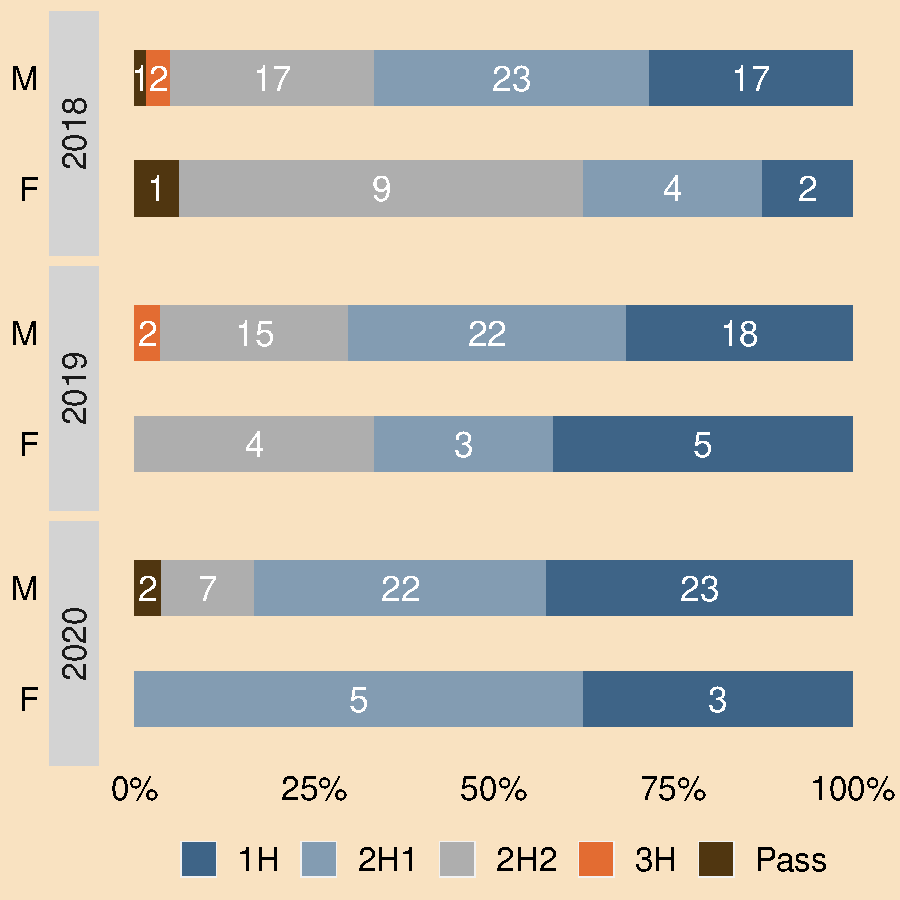
\includegraphics[width=2.7in]{fig/ug_attain2.pdf} % NEW
    \caption{Degree attainment BScCS}
    \label{fig:bsc:attainment}
    \end{subfigure}
    %\includegraphics[width=4in]{fig/bsc_attainment2.pdf} %% OLD
    %
    \begin{subfigure}[r]{2.7in}
    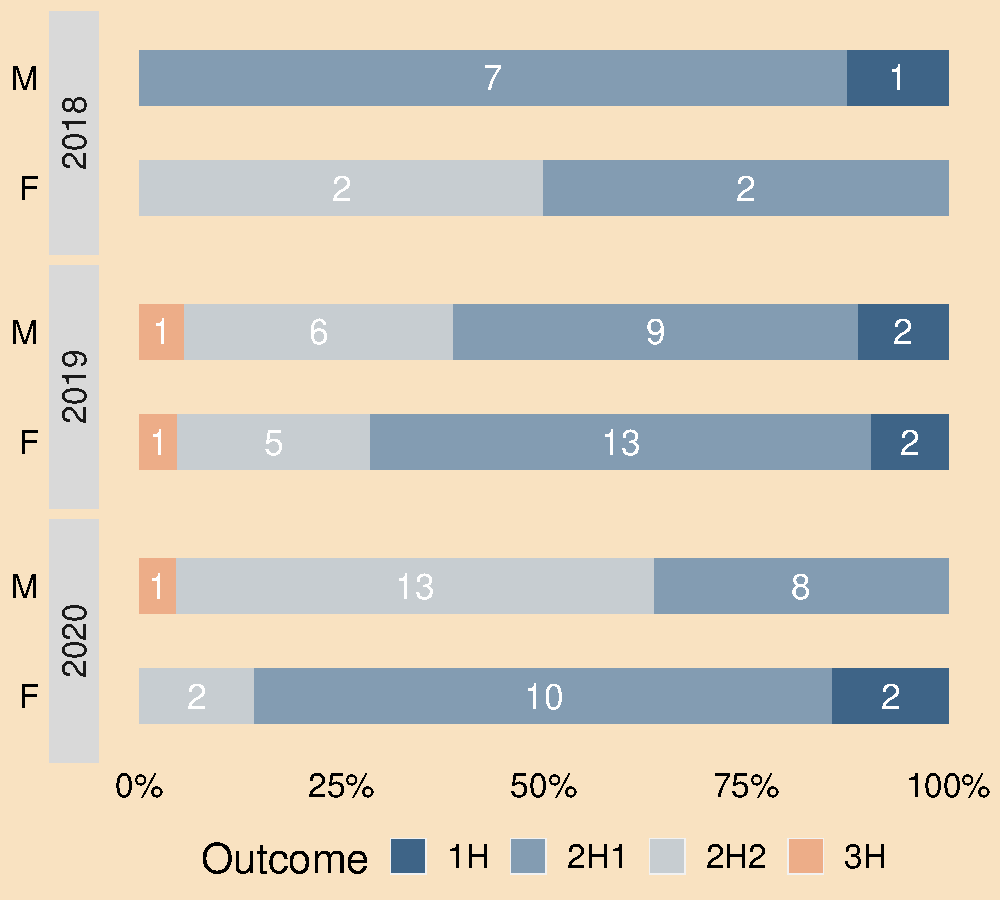
\includegraphics[width=2.7in]{fig/badhit_attainment2.pdf}
    \caption{Degree attainment BADHIT}
    \label{fig:badhit:attainment}
    \end{subfigure}
    %
    
    \label{fig:ug:attainment}
 \end{minipage}   
}
\end{figure}

% \begin{figure}[!tb]
%     %\centering
%     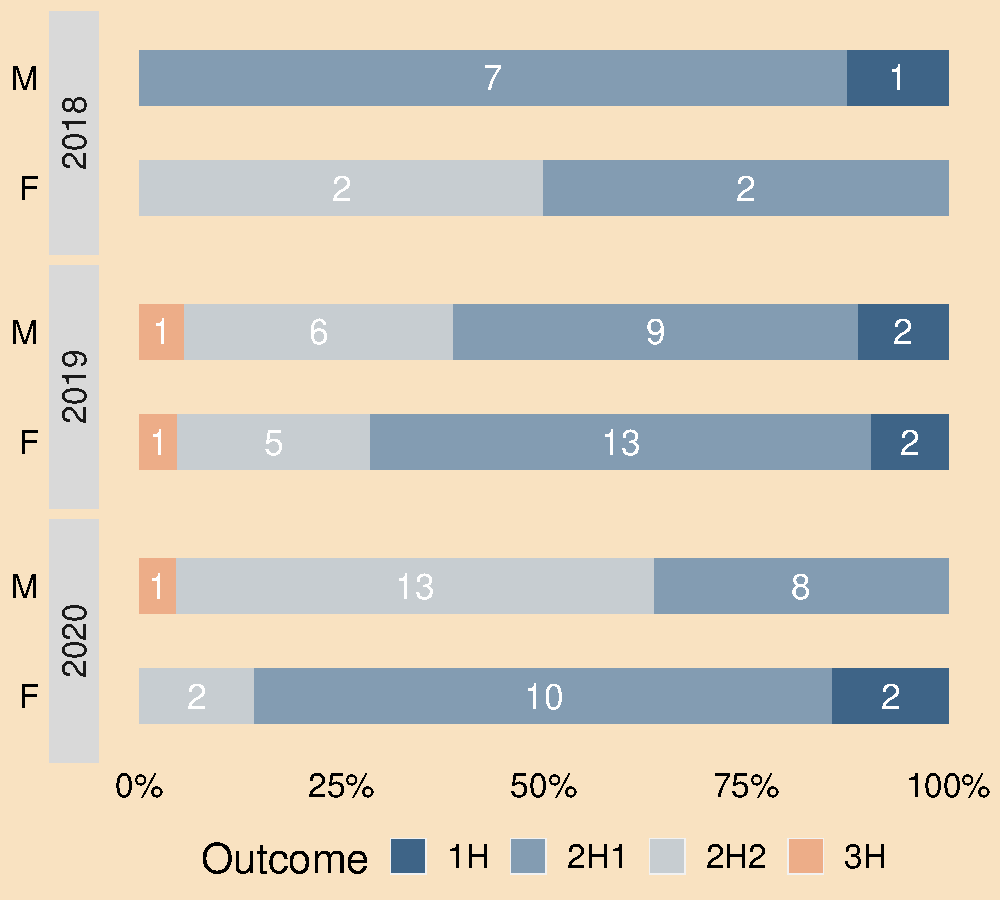
\includegraphics[width=4in]{fig/badhit_attainment2.pdf}
%     \caption{Degree attainment BADHIT}
%     \label{fig:badhit:attainment}
% \end{figure}

% \khcomment{Splice in 2022 attainment figure here. Add some comment.}
% 
% \khcomment{What can we say about gender and attainment?}

\subsubsection{Data on undergraduate students by gender and foundation courses}

The school does not offer any foundation courses.


\subsection{Analyse three years of data on postgraduate taught students by:} 
\instr{
\begin{itemize}
    \item gender and degree programme, with reference to discipline-specific benchmark data;  
    \item gender and degree attainment.  
\end{itemize}
}
\label{pg_data}


\subsubsection{Three years of data on postgraduate students by gender and degree 
programme}

% \akcomment{Section 2.1.c - omit comment on lack of availability of data on PGT 
% application/offer/acceptance rates - not asked for in the application form.   It 
% is implied that F representation at PGT level outperforms benchmark due to 
% higher % women on MSc CS and MScDSA (or am I misreading this?) Do we know if 
% other HEIs get fewer non-EU students in their PGT cohorts?
% }

% \khcomment{I'm not sure I understand what she means by the last
% sentence. Any ideas?
% }




Figure~\ref{fig:pg:enrolment} shows enrolment trends for the four taught
postgraduate programs listed in Table~\ref{tab:teachingportfolio} for the 
three-year period up to 2019-20.
The female participation rate for the  masters programmes are 
significantly better than for some of the undergraduate programmes.
Both the MSc in Computing Science and the MSc in Data Science have
a high proportion of non-EU students and \todo{while we do not have
concrete data on this it is noticeable that the gender balance for 
these two programmes is significantly healthier among the non-EU cohort.}
The MSc in Interactive Media (MScIM) is the one programme
across the entire portfolio where females (56-68\%)  
outnumber males.

\begin{figure}[!ht]
\colorbox{orangebg}{
\begin{minipage}{14.2cm}
    \caption{Enrolment postgraduate students 2017-2020}
    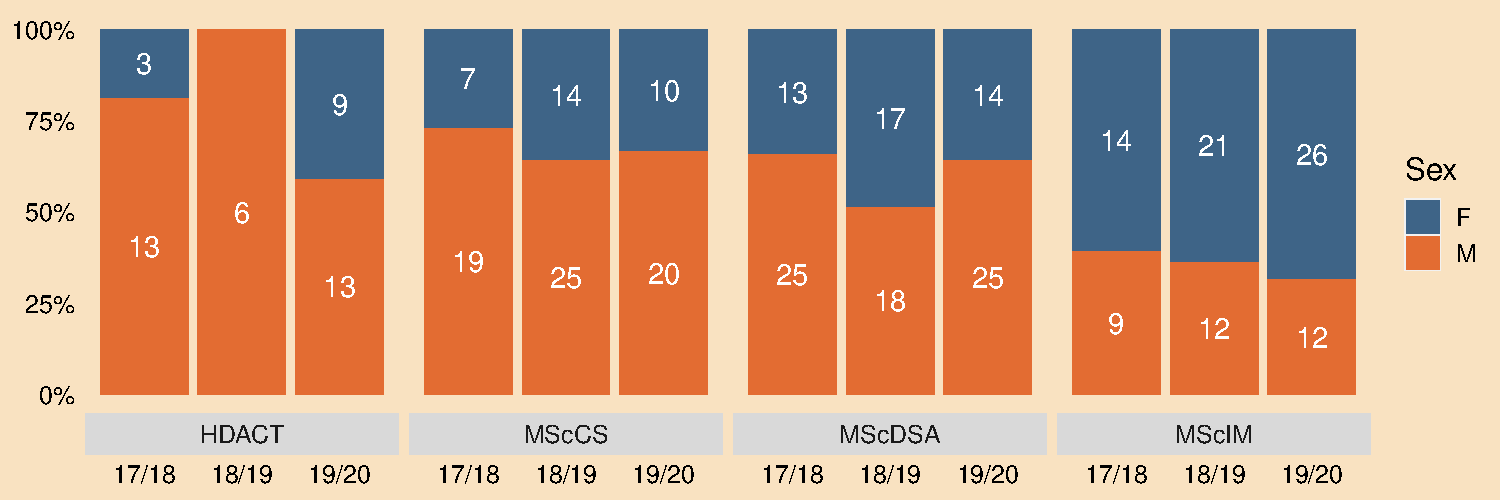
\includegraphics[width=\textwidth]{fig/pg_enrolment.pdf}
    
    \label{fig:pg:enrolment}
    \end{minipage}
}
\end{figure}


\begin{table}

\colorbox{SwanOrange!10}{
      \begin{minipage}{12cm}
      
\footnotesize       
\caption{Postgraduate male-female participation rates  benchmarked nationally
(HEA) and with the UK (HESA) (full-time students only)}
\label{tab:benchmarking:pg}

\sisetup{
    group-digits=all,
    group-minimum-digits=4,
    group-separator = {,},
    table-format=4.1,
    mode=text,
    reset-text-series = false, 
    text-series-to-math = true,
    reset-text-family = false, 
    text-family-to-math = true
}
\begin{tabular}{p{2cm} 
                S[table-format=3.1]
                S[table-format=3.1]
                S[table-format=3.0\%]
                p{0.7cm}
                S[table-format=3.1]
                S[table-format=3.1]
                S[table-format=3.0\%]
                p{0.7cm}
                S[table-format=4.1]
                S[table-format=5.1]
                S[table-format=3.0\%]}
\toprule
  & \multicolumn{3}{c}{\textbf{UCC CSIT}} 
  &
  &\multicolumn{3}{c}{\textbf{HEA (Ireland)}} 
  &
  &\multicolumn{3}{c}{\textbf{HESA (UK)}}\\
  \cmidrule{2-4}\cmidrule{6-8}\cmidrule{10-12}
Year & {F}& {M} & {F\%} & & {F}& {M}& {F\%} & & {F} & {M} & {F\%}\\ 
\midrule 
2017-18 &37 &63 &37\% && 173&414 &29\%  && 2790 &6520 &30\%\\
2018-19 &51 &62 &45\% && 209 &453 &32\% && 3563 &7870 &31\%\\
2019-20 &51 &67 &43\% && 289 &609 &32\% && 5560 &12950 &30\%\\
\bottomrule 
\end{tabular}
\end{minipage}
}
\end{table}



As Table~\ref{tab:benchmarking:pg} shows, 
our female participation rates have improved over the period 
presented for postgraduates overall from 37\% to 43\% and 
compare favourably 
with  Irish and UK benchmarks. For taught postgraduates CSIT's 37-45\%
is significantly above the HEA, HESA figures of 29-32\% and 30-31\%
respectively.



\subsubsection{Three years of data on postgraduate students by gender 
and degree attainment}

Figure~\ref{fig:pg:attainment} plots the degree classifications
achieved for those completing the four taught postgraduate 
programmes over the period 2018 to 2020. Because of the relatively
small numbers in some cohorts, there is some variation 
from year to year  and programme to programme, but no obvious
gender pattern is apparent, though as with the undergraduate
programmes, females feature prominently among those receiving 
higher grades.


\begin{figure}[!ht]
\colorbox{orangebg}{
\begin{minipage}{14.2cm}
 \caption{Degree attainment postgraduate students}
    %\centering
    \begin{subfigure}{2.8in}
    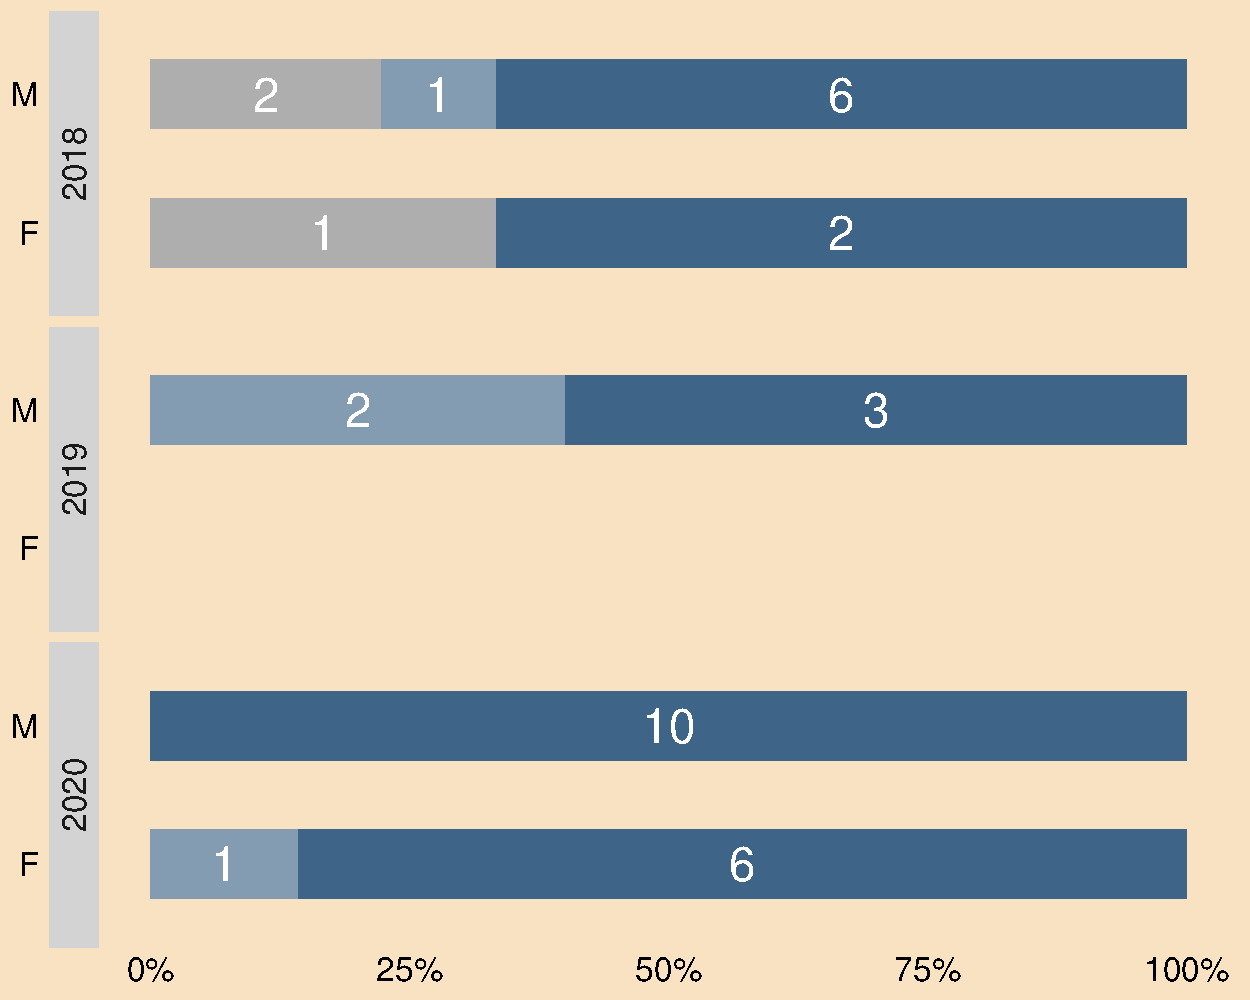
\includegraphics[width=2.8in]{fig/pg_hdact_attainment.pdf}
    \caption{Postgraduate attainment HDip ACT}
    \label{fig:hdip}
    \end{subfigure}
    %
    \begin{subfigure}{2.8in}
    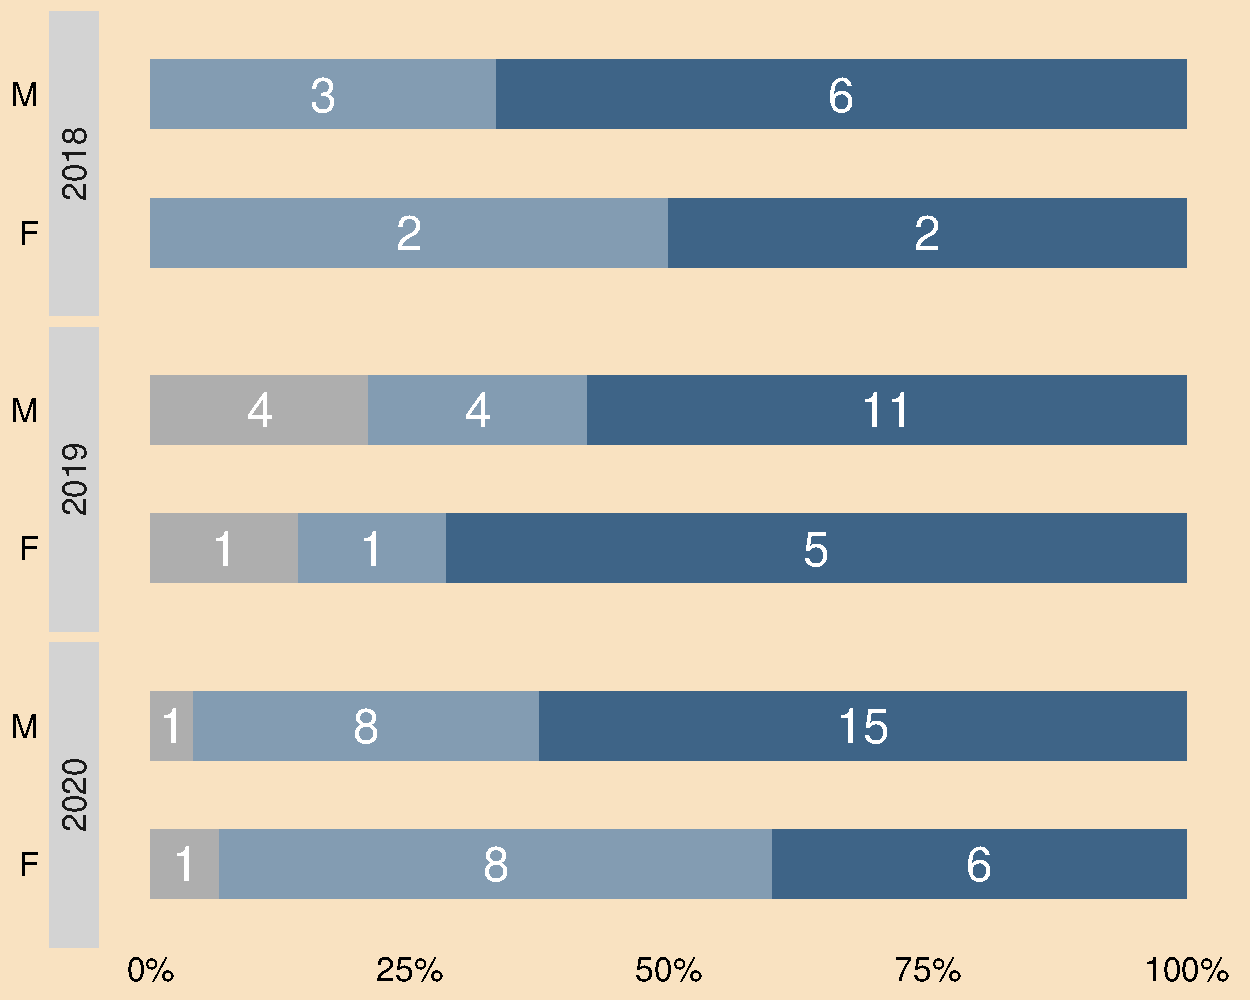
\includegraphics[width=2.8in]{fig/pg_msccs_attainment.pdf} 
    \caption{Postgraduate attainment MSc CS}
    \label{fig:msccs}
    \end{subfigure}
    %
    \par\bigskip
    %
    \begin{subfigure}{2.8in}
    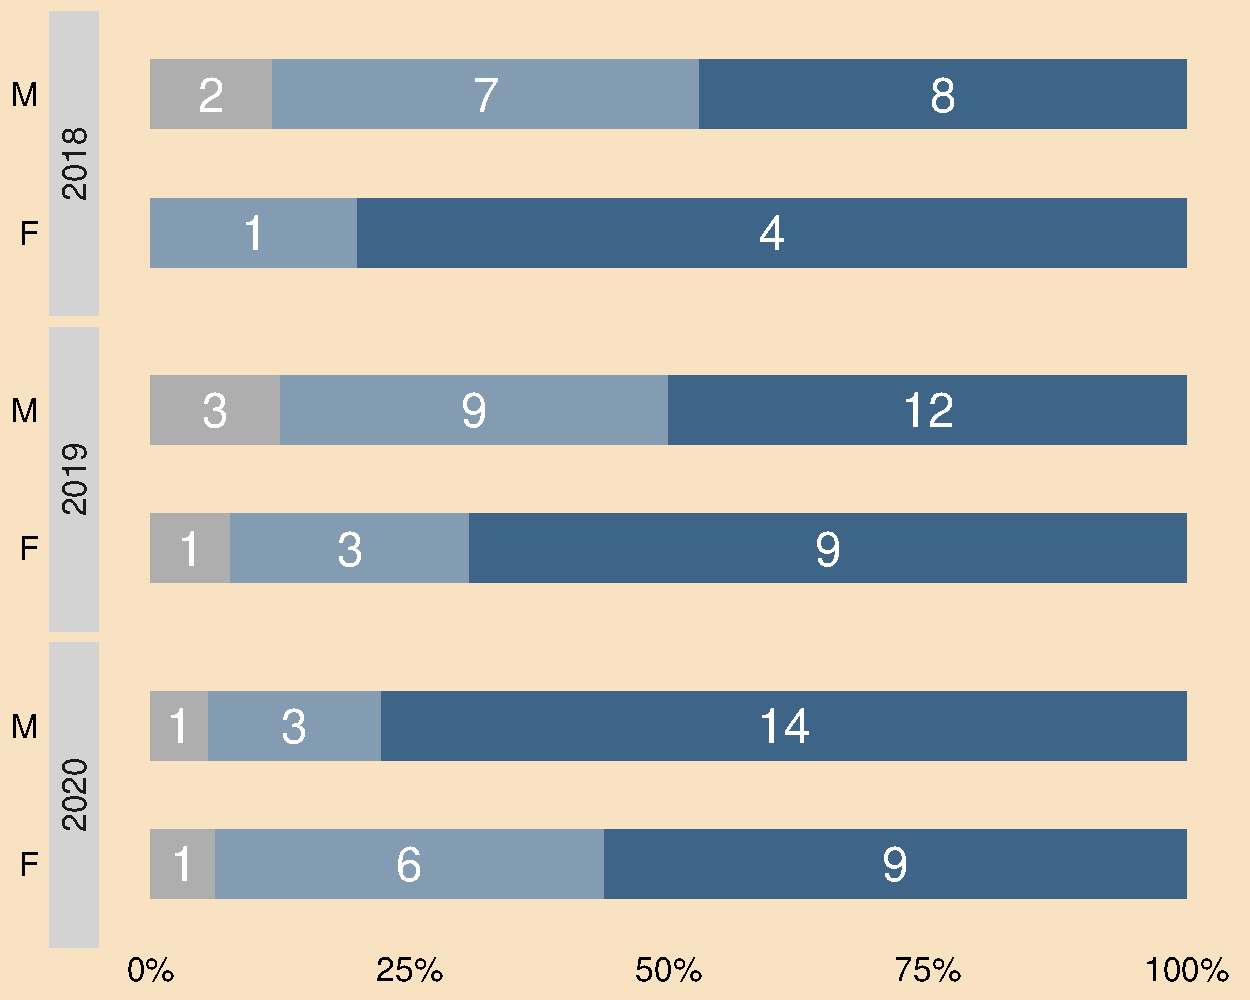
\includegraphics[width=2.7in]{fig/pg_mscdsa_attainment.pdf} 
    \caption{Postgraduate attainment MSc DSA}
    \label{fig:mscdsa}
    \end{subfigure}
    %
    \begin{subfigure}{2.8in}
    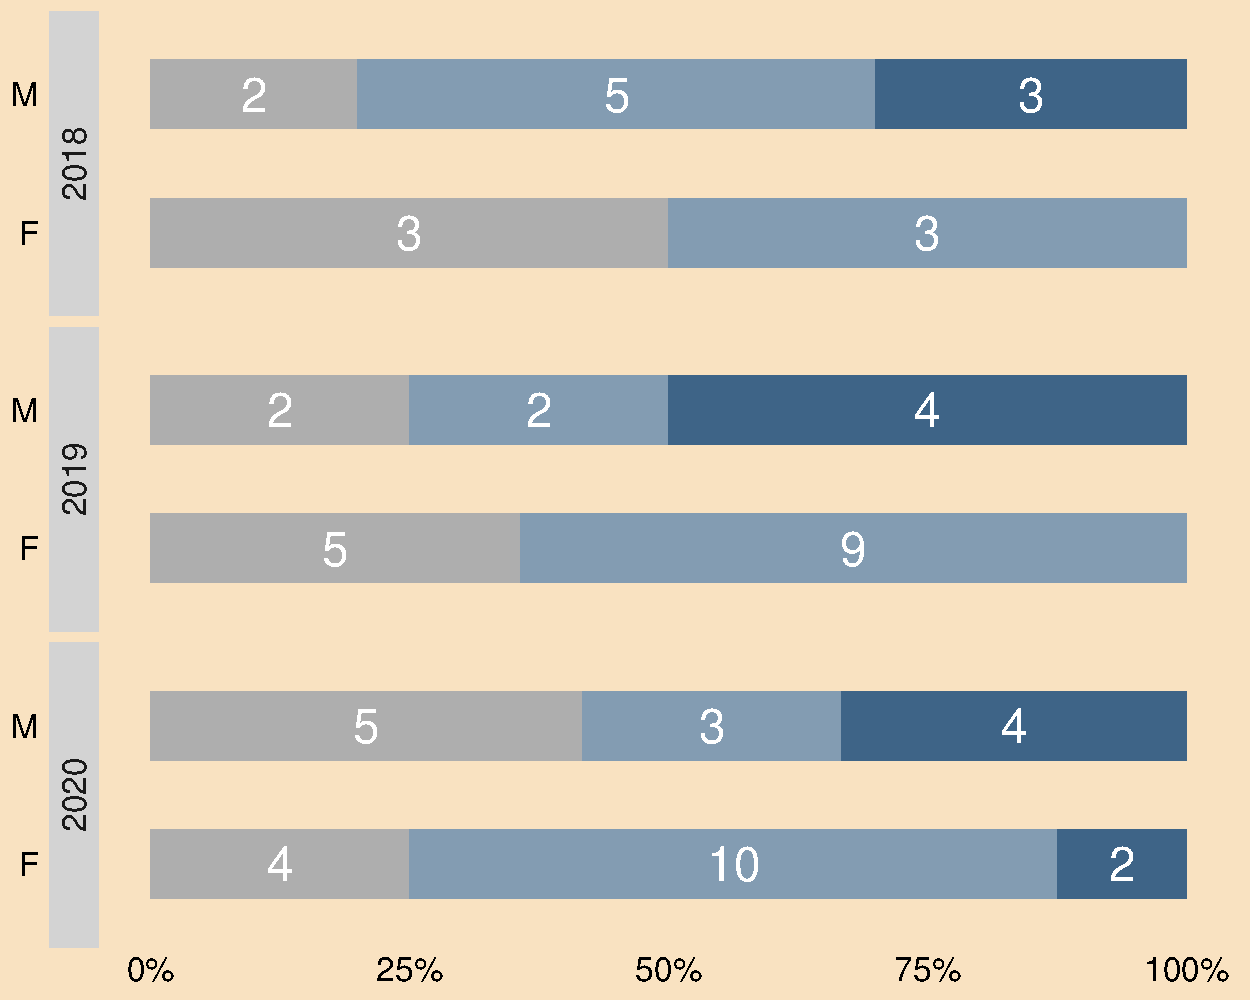
\includegraphics[width=2.7in]{fig/pg_mscim_attainment.pdf} 
    \caption{Postgraduate attainment MSc IM}
    \label{fig:mscim}
    \end{subfigure}
    %
    \par 
    %% Add the legend
   
    \begin{subfigure}{14cm}
    \centering 
    % left bottom right top
    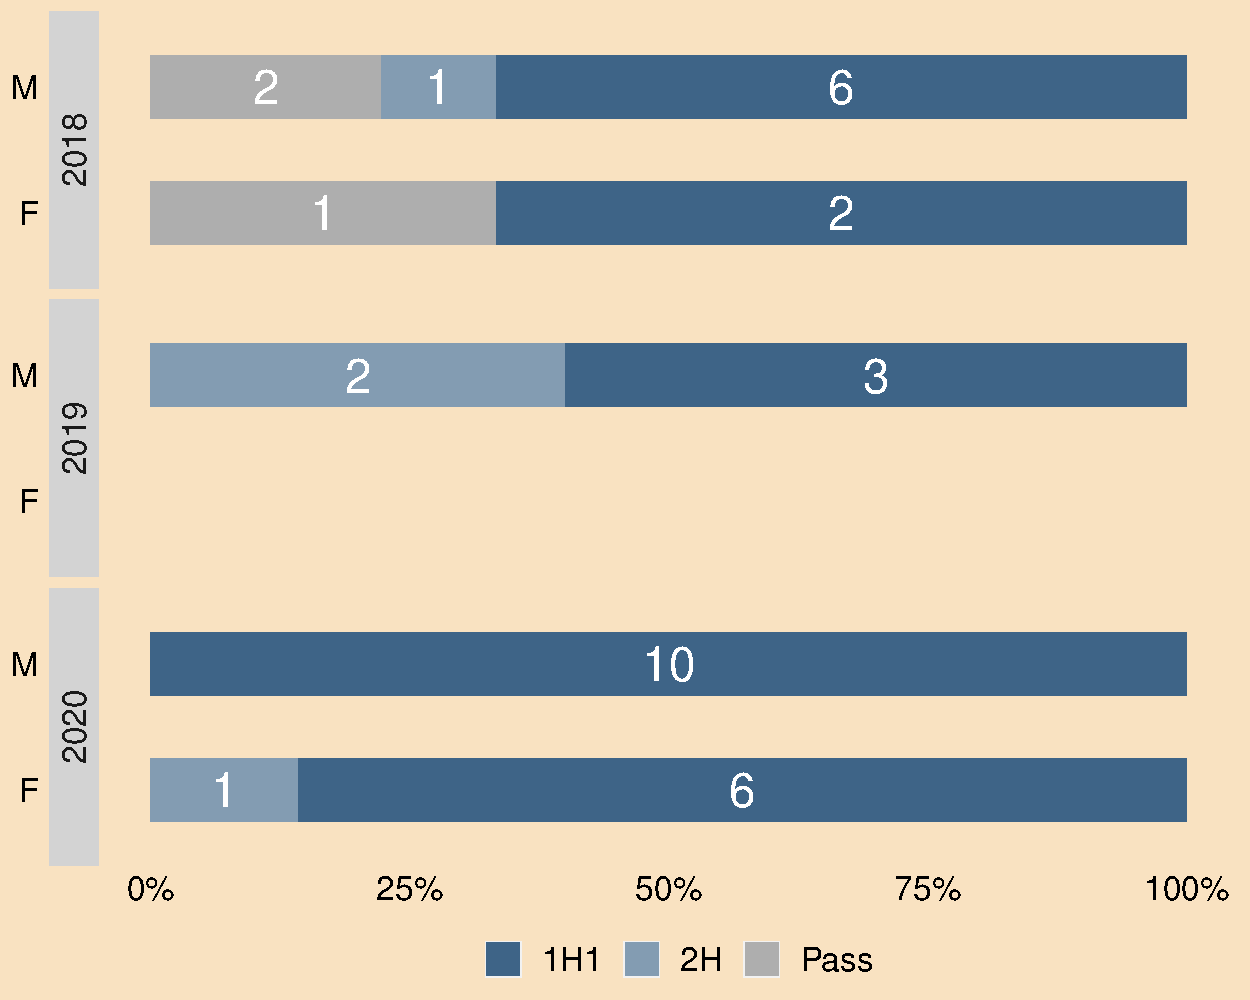
\includegraphics[trim={0 0 0 15.5cm},clip,width=3in]{fig/pg_legend.pdf} 
    \end{subfigure}
    
    \label{fig:pg:attainment}
\end{minipage}
}
\end{figure}


\subsection{Analyse three years of data on postgraduate research 
students by:}  
\instr{
\begin{itemize}
    \item gender and enrolment; 
    \item gender and application, offer, and enrolment, with comment on how this data is collected and evaluated by the department, and on any gender disparities in student funding;  
    \item gender and completion rates.  
\end{itemize}
}
\label{sec:phdstudents}


\subsubsection{Three years of data on postgraduate research students 
by gender and enrolment}
\label{sub:phdnumbers}

% \akcomment{PGR - discussion of data by (a) gender and enrolment and (b) gender 
% and completion rates, is mixed up - suggest separating these out.  Comment on 
% gender differences in enrolment rates (if any).  It's observed that a 40% 
% recruitment quota for CRT PhDs "has driven an increase in F PhD intake since 
% 2019" - not evident in Fig. 2.7?  Does the quota account for the statement that 
% "intake in recent year has been much more balanced" - or are there other 
% factors? Panellists may be interested in understanding what the learning has 
% been from this experience?  Reflection/comment is needed on why UCC below 
% benchmark w/r/t PhD enrolment (Tables 2.6, 2.7).   Actions 2.1.5 - 2.1.5 can be 
% cited here but might be better treated more fully in section  2.1.e
% }

Figure~\ref{fig:phdenrolments} summarises the numbers of students 
enrolled as PhD students 2017 to 2000. The total numbers enrolled fell from 40 in 2017 to 32 in 2019,
reflecting the ending of one funding stream, before increasing 
again to 41 in 2019 as the CRTs were introduced that year.

\begin{figure}[!ht]
\colorbox{orangebg}{
\begin{minipage}{14.2cm}
    \caption{Total enrolment numbers of PhD students (2017-2020)}
    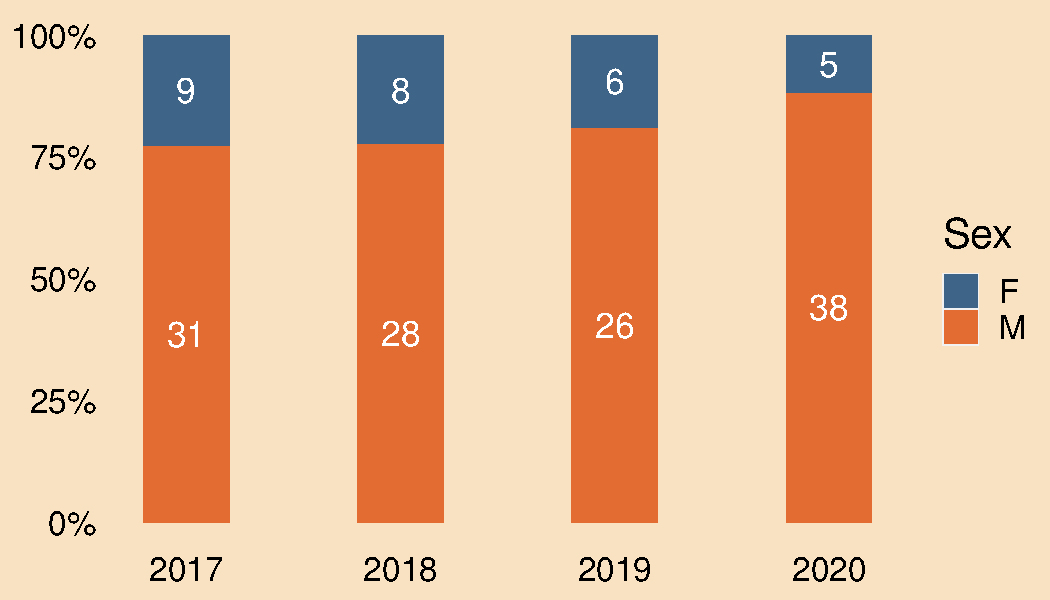
\includegraphics[width=4in]{fig/phd_registered.pdf}
    \label{fig:phdenrolments}
    \end{minipage}
}
\end{figure}

% \khcomment{Replace by data from Table K from EDI spreadsheet? 
% }
% 
% \khcomment{If CRTs started in 2019 why did numbers fall in 2020?
% }




\todo{
It is noteworthy that females were proportionately
well represented among those completing PhD from 2018 onwards.
The fall in female PhD registrants from 2019 to 2020 may in
part be explained by the fact that there were six females
registered in 2019 and three females completions that year.
}
%[DT: Verify from PhD spreadsheet]

In 2019 the school received SFI funding for two Centres for Research 
Training (CRT). These CRTs have explicit targets for 
increased female PhD students (40\%), which has driven an 
increase in the intake of female PhD students in the school 
since 2019. This trend has been continuing since as we are 
recruiting a total of 48 PhD students into the school through 
this mechanism over the life of these CRTs. As SFI has
gender targets attached to other funding, a similar pattern 
is expected among the non-CRT PhD intake in future years.

\todo{
Invariably, PhD students are funded in full either through one 
of the CRTs or by research funds awarded to their supervisor 
or the research centre to which they are affiliated. The 
funding profile by gender mirrors the enrolment profile.
}
% Table~\ref{tab:benchmark:phd} presents some PhD registration
% data for various Irish universities for the period
% 2018-19 to 2020-21. The data for other institutions 
% was sourced from HEA. It should be noted that while
% some institutions have higher PhD numbers overall,
% these are generally far larger departments in terms of 
% academic staff.
% 
% \khcomment{Verify this. BOS feels it looks wrong.}
% 
% \begin{table}[!ht]

\colorbox{orangebg}{
      \begin{minipage}{14.2cm}
\caption{PhD Registrations in Irish Universities 2018-19 to 2020-21}
\label{tab:benchmark:phd}
\footnotesize 

\sisetup{
    group-digits=all,
    group-minimum-digits=4,
    table-format=2.1,
    mode=text,
    reset-text-series = false, 
    text-series-to-math = true,
    reset-text-family=false, 
    text-family-to-math=true
}


\begin{tabular}{p{5.5cm}
                R{1.3cm}
                R{1.3cm}
                !{\quad}
                R{1.3cm}
                R{1.3cm}
                !{\quad}
                R{1.3cm}
                R{1.3cm}}
\toprule 
Institution & 
\multicolumn{2}{c}{2018-19} &
\multicolumn{2}{c}{2019-20} &
\multicolumn{2}{c}{2020-21} \\
\cmidrule(l){2-3}\cmidrule(l){4-5}\cmidrule(l){6-7}
& Total & \%F & Total & \%F & Total & \%F \\ 
\midrule 
Dublin City University (DCU)&
54& 39&
53& 38&
69& 35\\
Maynooth University (MU) &
25& 32&
25& 36&
19& 26\\
Trinity College Dublin (TCD) &
92& 38&
87& 32&
104& 36\\
University College Cork (UCC)&
36& 22&
32& 19&
43& 11\\
University College Dublin (UCD)&
104& 29&
125& 35&
134& 36\\
University of Limerick (UL)&
46& 20&
41& 10&
33& 15\\
\bottomrule 

\end{tabular}

\end{minipage}
}

\end{table}
% \khcomment{PhD benchmarking table removed; can we get some
% reliable PhD numbers for other institutions?
% }

While the percentage of females among PhD students was historically 
low,  the intake in recent year has been much more balanced as 
demonstrated by Table~\ref{tab:phdintakerecent}. Note that these
numbers relate those in their first year of their PhD, whereas the 
registration numbers in Figure~\ref{fig:phdenrolments} include students  in all years of their studies.

\input{tables2/tab_phd_intake_recent_modified}

% \khcomment{Can we add 2022-23 numbers for completeness. Why the
% big drop in 2021-22? From next table it should be M = 42,
% F = 21, F\% = 33?
% }


\begin{table}[!htb]
\colorbox{SwanOrange!10}{
      \begin{minipage}{14.2cm}
\caption{PhD students registered 2022-23
by centre and gender}
\label{tab:phdregistrations2223}
\footnotesize 

\sisetup{
    group-digits=all,
    group-minimum-digits=4,
    mode=text,
    reset-text-series = false, 
    text-series-to-math = true,
    reset-text-family=false, 
    text-family-to-math=true
}


\begin{tabular}{p{6cm}
                R{1cm}
                R{1cm}           
                R{1cm}
                R{1cm}
                }
\toprule                 
\textmd{Research Centre}&
\textmd{M}&
\textmd{F}&
\textmd{Total}&
\textmd{\%F}\\ 
\midrule 
Advance-CRT&
12& 8& 20& 40\%\\
AI-CRT&
8& 4& 12& 33\%\\
Insight/ Confirm&
11& 5& 14& 36\%\\
MISL, Confirm, Lero, Enable, \todo{PCAV} &
8& 4& 12& 33\%\\
Other&
3& 0& 3& 0\%\\ 
\midrule 

Total&
42& 21& 63& 33\%\\

\bottomrule 
\end{tabular}

\end{minipage} 
}

\end{table}




% \khcomment{Clarify presence of Confirm twice. May need to
% add MISL and PCAV to earlier table.
% }


\subsubsection{Three years of data on postgraduate research students by gender, 
application, offer, and enrolment}
\label{sec:phdnumbers}

% \akcomment{Section 2.1.d - 1. data on application, offer, enrolment incomplete; 
% application questions on how this data is collected and evaluated by the School 
% need to be addressed; also the question seeking comment on gender disparities on 
% student funding needs to be addressed. 2. PGR completion rates - comment is 
% needed on gender differences in completion rates (if any). Completion rates are 
% calculated based on corresponding intake data - do you have this?  Only on-time 
% completion data is provided here, but it's difficult to contextualise without 
% access to completion rates.
% }


Historically, the PhD application process was handled by individual 
PIs/groups and while larger groups such as Insight has maintained
records relating to its students, no records were maintained at 
school level to monitor the overall gender breakdown of the number 
of applicants, offers and acceptances. Indeed, gender information was
often not requested of applicants. 

As noted earlier, the CRTs do have an explicit gender targets for enrolment.
Table~\ref{tab:crtapplications} summarises the
number of applications and enrolments by gender for the two CRTs
since their introduction in 2019. Note that the CRTs are national
consortia with five partner institutions each. The application
process is handled at consortium level and matched with specific
institutions and supervisor subsequently. Hence, it is not possible
to disaggregate applications by institution.

\input{tables2/tab_crt_applications_new}


For the years 2019, 2020 and 2021 the percentage 
of females among the applicants ranged from  38\% to 27\% for the 
Advance CRT and from 25\% to 31\% for CRT-AI. The percentages for 
successful applicants ranged from 45\% to 39\% and 31\% to 49\%, 
respectively. For both CRTs the percentage of successful
females exceeded the percentage among the applicant pool.



% \newcommand{\actdeptcareerchoice}{
% Survey final year UGs to ascertain career choices and to probe attitudes to 
% research and academic careers.
% }
% \begin{action}[label=action:dept:careerchoice]{}
% \actdeptcareerchoice
% \hfill{
%     \hypersetup{hidelinks}
%     \hyperlink{b4}{\gotoactionsymbol{}}
% }
% \end{action}


% \newcommand{\actdeptpromisingfemale}{Approach promising female final year undergrads to encourage considering PhDs.
% }
% \begin{action}[label=action:dept:promisingfemales]{}
% \actdeptpromisingfemale
% \hfill{
%     \hypersetup{hidelinks}
%     \hyperlink{b5}{\gotoactionsymbol{}}
% }
% \end{action}


% \newcommand{\actdeptringfence}{
% Establish fund to support some undergraduate research internships opportunities; 
% ringfence a proportion for females targeting at female undergraduates.
% }
% \begin{action}[label=action:dept:ringfence]{}
% \actdeptringfence
% \hfill{
%     \hypersetup{hidelinks}
%     \hyperlink{b6}{\gotoactionsymbol{}}
% }
% \end{action}

% \newcommand{\actdepthighlight}{
% Highlight female researchers and their work more 
% prominently on promotional materials, webpages and so on.
% }
% \begin{action}[label=action:dept:highlight]{}
% \actdepthighlight
% \hfill{
%     \hypersetup{hidelinks}
%     \hyperlink{b7}{\gotoactionsymbol{}}
% }
% \end{action}


\subsubsection{Three years of data on postgraduate research students by gender 
and completion rates}

Figure~\ref{fig:phdcompletions} shows the number of PhD
completions for the period 2017-20.
Table~\ref{tab:phdcompletion} presents completion time data for 
males and females for those who graduated within the time-frame 
2017-18 to 2019-20.
Times are rounded to nearest year. This is based on registration
and graduation data. As there is often a time lag between ``finishing
up'' (viva voce, submission) and graduation, these figures may overstate 
the amount of time to complete by a few months in some cases.


\begin{figure}[!tb]
  \colorbox{orangebg}{
    \begin{minipage}{14.2cm}
        \caption{Number of PhD  completions (2017-2020)}
        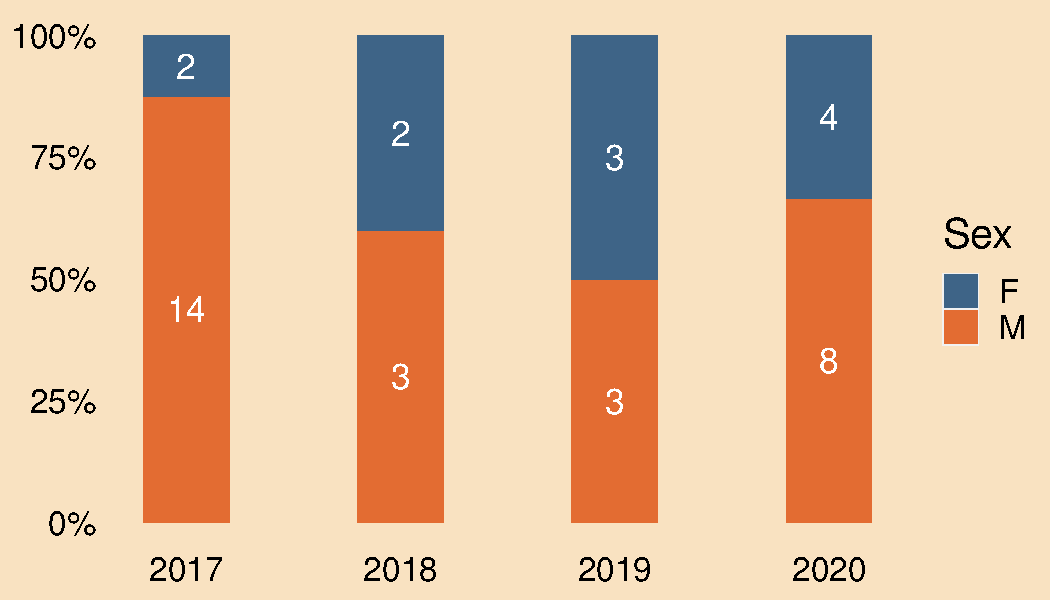
\includegraphics[width=4in]{fig/phd_completions.pdf}
        \label{fig:phdcompletions}
    \end{minipage}
    }
\end{figure}



\input{tables2/tab_phd_completion}


It appears that the completion time is somewhat worse for females.
While most students required more than four years to complete,
three out of seven females took six years or more, whereas the
corresponding figure for males was seven out of 23. 
\todo{This need further investigation.}

% \khcomment{What is the funding situation for those students
% taking more than four years?
% }
% 
% 
% \khcomment{Need something on completion *rates* i.e. how many
% who started did not finish or left with a masters and whether
% there is any gender pattern to be observed.
% }

\subsection{Comment and reflect on the relationship (if any) between the department’s outreach, engagement, and support activities and issues or opportunities in the student pipeline. This should include comment on how the department recognises staff and student contributions to these activities and monitors the gender balance of those involved.}

% \akcomment{need to focus more closely on the question asked here.  Suggest you 
% first summarize the key issues in the student pipeline identified in Sections 
% 2.1b - d; e.g., list them - then comment on how the School's outreach, 
% engagement and student support activities can be used to deliver interventions 
% (actions) that will address these challenges.  (Clarity needed on how Actions 
% 2.1.9 and 2.1.10 respond to the analysis in this section).
% }
% 
% \khcomment{Try to reflect Anne's suggestions here. Her takes seems to be
% that we have missed the point completely. So this sectio
% may need a complete rewrite. 
% }

The school is involved in several outreach initiatives for prospective undergraduate
students. Apart from its participation in University events such
as open days and careers guidance information sessions, the School
hosts a number events and activities of its own such as an annual
information evening, a programme of weekend programming activities
and summer camps both aimed at second-level students. Academic staff also make targeted school visits with an increased focus in
recent years on girls schools.

A range of  measures are in place to ensure undergraduate students
are supported during their time with us. This includes a mentoring
scheme for first-year students, a team of programme directors
and year heads to offer advice, support
and guidance to students.

While all these activities are valuable in themselves, they have 
evolved in a piecemeal fashion. A useful outcome of the self-assessment is the realisation that we have never conducted
a comprehensive audit of existing activities to assess their 
effectiveness and reflect on how they might be reconfigured 
to mitigate the two key challenges in the student pipeline:
(1) the under-representation of females in certain undergraduate
programmes especially the BSc in Computer Science, and 
(2) the comparatively small number of female undergraduates
who opt to progress to graduate research studies.


Our response to the former is twofold: to undertake a 
root-and-branch review of existing marketing and outreach
activities and also to re-imagine how the School presents
itself across all media to help counter the negative image
computer science seems to have as a discipline  among young
women (see Actions~\ref{action:review:outreach} and \ref{action:materials:guidelines}).



\newcommand{\actreviewoutreach}{Review existing  marketing, outreach, engagement and support activities to better encourage female school leavers to choose CS and  improve the experience of those that  do.}
\begin{actionblock}{\ksspace{}Review Marketing and Outreach Materials}{review:outreach}
\actreviewoutreach 
\hfill{
    \hypersetup{hidelinks}
    \hyperlink{b0}{\gotoactionsymbol{}}
}
\end{actionblock}



\newcommand{\actmaterialsguidelines}{Develop guidelines to inform production of all future materials and visuals in order to project the school in as EDI-friendly a light as possible across  all channels; apply these to revamp all promotional/marketing, recruitment materials, web and social media channels over lifespan of award.}
\begin{actionblock}{\ksspace{}Develop EDI-Friendly Guidelines}{materials:guidelines}
\actmaterialsguidelines
\hfill{
    \hypersetup{hidelinks}
    \hyperlink{b0}{\gotoactionsymbol{}}
}
\end{actionblock}



Persuading young female undergraduates to consider a research career will be a significant challenge for the sort of economic and career factors outlined in Section \todo{XX}. However, we believe that  by providing a more engaging and supportive environment for females, including opportunities to engage with research as undergraduates through internships, for example, will help stimulate interest. 
The appointment of a designated staff member to lead these efforts
will be essential (see Action~\ref{action:edi:coach}).


\newcommand{\actedicoach}{Appoint an EDI coach to coordinate EDI efforts relating to female undergraduate students, including outreach and recruitment, mentoring, ongoing supports etc.}
\begin{actionblock}{\ksspace{}Appoint EDI Coach}{edi:coach}
\actedicoach 
\hfill{
    \hypersetup{hidelinks}
    \hyperlink{b0}{\gotoactionsymbol{}}
}
\end{actionblock}



\newcommand{\actsurveyfemales}{Survey existing undergraduate females to gauge attitudes and perceptions towards 
research/academic careers.}
\begin{actionblock}{\ksspace{}Investigate Attitudes and Perceptions towards Academic Careers}{survey:females}
\actsurveyfemales
\hfill{
    \hypersetup{hidelinks}
    \hyperlink{b0}{\gotoactionsymbol{}}
}
\end{actionblock}


\newcommand{\actencouragefemales}{Proactively engage with talented female undergraduates to encourage greater uptake of PhD studies.}
\begin{actionblock}{\ksspace{}Encourage Female Undergraduates to Pursue PhD studies}{encourage:females}
\actencouragefemales 
\hfill{
    \hypersetup{hidelinks}
    \hyperlink{b0}{\gotoactionsymbol{}}
}
\end{actionblock}


% Template for KJS actions cloned from "old" action in Draft 1.
% included here to simplify the action-fication of the new acton
% below. 
%
\newcommand{\actenrichopportunities}{Enhance enrichment opportunities for female undergraduates to gain work experience aligned with roles in which females are underrepresented such as IT support work  with school’s systems support unit, research internships with school’s research centres or independent study research-focused modules for gifted students.}
\begin{actionblock}{\ksspace{}Enrich Opportunities for Female Undergraduates}{enrich:opportunities}
\actenrichopportunities
\hfill{
    \hypersetup{hidelinks}
    \hyperlink{b0}{\gotoactionsymbol{}}
}
\end{actionblock}


\newcommand{\actboostvisibility}{Boost visibility of females  and highlight their work to provide role models at all levels.}
\begin{actionblock}{\ksspace{}Boost Visibility of Females}{boost:visibility}
\actboostvisibility
\hfill{
    \hypersetup{hidelinks}
    \hyperlink{b0}{\gotoactionsymbol{}}
}
\end{actionblock}



\subsection{Provide data for academic and research staff by gender and grade. Analyse and benchmark the career pipeline.}
\label{sec:academic_research}

% \akcomment{1. present benchmark data in a table rather than just in narrative 
% form (p. 32). 2. Fig. 2.8 - table header refers to UG but only PhD data included 
% (suggest including UG, PGT, PGR student data). Give year of data reported.  
% Consider scissors graph? 3. 3 "choke points" in career pipeline are identified 
% on p. 34. Distil the discussion of these choke points.   The concluding sentence 
% suggests that recruitment and promotion actions will improve the gender balance 
% over time.  More specificity here would be useful, e.g do those actions 
% specifically target one or more of these choke points?  If so, how?
% }

Table~\ref{tab:acresstaff} presents data for academic staff and researchers
by gender and grade. 
The researchers category includes only those in direct research roles:
those in research support roles are included below with other professional, 
managerial and support staff. Dashes denote zero values.

\begin{tabbox}[10cm]{!b}
\caption{CSIT academics and researchers (2020)}
\label{tab:acresstaff}
\footnotesize 

      
\begin{tabular}{p{4cm}
                C{1cm}
                C{1cm}
                c
                p{0.7cm}
                C{1cm}
                C{1cm}
                c}
\toprule 
%\multicolumn{7}{c}{\bfseries Academics and Researchers (2020)}\\ \hline
  & \multicolumn{3}{c}{Permanent/CID} && \multicolumn{3}{c}{Fixed-Term}\\
  \cmidrule{2-4}\cmidrule{6-8}
  Grade & {F} & {M} & \%F && {F} & {M} & \%F\\
  \midrule 
 
  Professor& -& 4& -&&- &- &- \\
  \hdashline 
  Professor (Scale 2) &- & 4&- &&- &- &- \\
  \hdashline 
  Senior Lecturer &-& 5&- &&- &- &- \\
  \hdashline 
  Lecturer (above bar)&1 &14 &7\% &&- & 1&- \\
  \hdashline 
  Lecturer (below bar)&1 &-& 100\% && 1&2 & 33\%\\ 
  
\midrule 
Research staff*\\
\midrule 
 Senior Research Fellow&- &- &- &&- & 1&-\\
 \hdashline 
 Research Fellow &- & -&- &&- &3 &-\\
 \hdashline 
 Senior Postdoc &- &- &- &&- &4 &- \\
 \hdashline 
 Postdoc & - &- &- &&3 &10 & 23\%\\
 \hdashline 
 Research Assistant &- &- &- && 1&1 & 50\%\\
\bottomrule 
\end{tabular}
\\[2mm]
{\sffamily * Research staff are hired on fixed-term contracts only.}


\end{tabbox}



The gender imbalance is stark for both academic and researcher
categories, most acutely at senior levels. There are no females 
at Senior Postdoctoral level or above  and none at Senior Lecturer level or above. 


Table~\ref{tab:academic_benchmark} compares CSIT's academic
staff profile with that of two peer institutions, \ac{UCD} and \ac{TCD}.
\todo{This information is retrieved from these schools' webpages at the time 
of writing, hence the slight differences between the UCC 
numbers quoted here and those given earlier.} 
The percentage of female academics at CSIT is just below 10\%, 
which compares unfavourably with 16\% and 29\% at UCD and TCD 
respectively. There are no females at UCC at Senior Lecturer
level or above, compared with six out of 58 at UCD and five 
out of 59 at TCD.
% The TCD numbers
% include some statisticians, who are also members of their school.
% As the webpages do not distinguish between lecturers above and 
% below the merit bar, or between levels of those bearing the 
% title ``Professor'' we report both professors and lecturers
% each on a single line.

%
% Have tried to replicate your table style using 
% 'tab_taught_programmes as a model.
%

% Material from here to 'preamble' marker below copied
% verbatim from model aprt from caption and label.
%
\begin{table}[!htb]
\colorbox{SwanOrange!10}{
      \begin{minipage}{14.2cm}


\caption{Academic staff by grade and gender benchmarked against
peer institutions (September 2022)}
\label{tab:academic_benchmark}
\footnotesize 

\sisetup{
    group-digits=all,
    group-minimum-digits=4,
    mode=text,
    reset-text-series = false, 
    text-series-to-math = true,
    reset-text-family=false, 
    text-family-to-math=true
}
% 'preamble ends here'

                
\begin{tabular}{p{7.3cm}
                C{1cm}C{1cm}
                p{.5cm}
                C{1cm}C{1cm}
                p{.5cm}
                C{1cm}C{1cm}
               }
\toprule
&
\multicolumn{2}{c}{\textmd{UCC}}&&
\multicolumn{2}{c}{\textmd{UCD}}&&
\multicolumn{2}{c}{\textmd{TCD}}\\
\cmidrule(l){2-3}\cmidrule(l){5-6}\cmidrule(l){8-9}
Grade & M & F && M & F && M & F\\
\midrule 
Professors&
9 & - & &7 & 3 && 10 & 3\\
Senior Lecturer &
4 & - & &17 & 3 && 9 & 2\\
Lecturer&
16 & 3 && 25 & 3 && 23 & 12\\
\midrule
Subtotal Senior Lecturer or above&
13 & - && 24 & 6 && 19 & 5\\
Total&
29 & 3 && 49 & 9 && 42 & 17\\

% Material from here on copied verbatim from model.
\bottomrule 
\multicolumn{6}{l}{UCD: University College Dublin, TCD: Trinity College Dublin}\\
\end{tabular}
{\sffamily
Note: The TCD numbers include some statisticians, who are also members of their school. The source of these data does not distinguish between Lecturers above and 
below the merit bar, or between levels of those bearing the 
title `Professor.'}\\
\end{minipage} 
}

\end{table}

% Notes:
% Scraped from webpage except
% Andrea and Harry added




The \ac{HESA} data  (2019-20 ICTS) from the UK indicates 16\% professors in 
computer science are females and 22\% of all research and academic staff 
excluding professors.

% \khcomment{Can we scrape info from websites? Or what about their 
% AS applications? NB: TCD website also has sysadmin staff might be
% useful as benchmark in that section.
% }

The poor gender balance among academic staff in CSIT is largely 
a reflection of the uneven pattern of recruitment over the past 
twenty-five years. 
A rapid expansion in numbers in the 1990s and early 2000s was
followed by a long hiring drought. Prior to 2017 no permanent
academic appointment had been made since 2004, essentially 
locking in a historical imbalance. It was not until 2017 that
the first female permanent member of academic staff was appointed.
% Note 2017: AOD, AZ, KJS & PP joined
% 2004: GP joined and none in intervening period.

However, since 2017 CSIT has filled 13 permanent academic posts 
(nine male and four female), two of whom (one male, one female)
have since resigned to take up posts abroad.
%male: KJS, AZ, PP, AA, UR, DP, HC, AV, Harry
%females: AOD, LC,  LM, RM
While this is a step in the right direction, the School realises that much work remains to be done to achieve a healthy gender balance, and
%The healthier gender balance evident in recent hires is a positive development and a trend 
we will actively strive to continue in
the years ahead through the adoption of gender-positive recruitment
measures. 
% \khcomment{Update figures wrt 2022 hires}

In the years up to 2027, 12 staff (nine academic, three administrators) are
expected to reach the normal retirement age. Some new posts
are also expected based on increasing student numbers. % from new programmes.
This significant tranche of staff openings over the coming years
presents an opportunity to approach recruitment in a more coordinated 
strategic manner, not least in using the opportunity to further 
improve gender balance. 

Figure~\ref{fig:pipeline} presents the percentage of females
from undergraduates to professors. 

\begin{figure}[!ht]
    \colorbox{orangebg}{
    \begin{minipage}{14.2cm}
    \caption{Career pipeline 2020: gender distribution across academic levels 
of seniority, from PhD student to Senior Lecturer (SL) and above}
    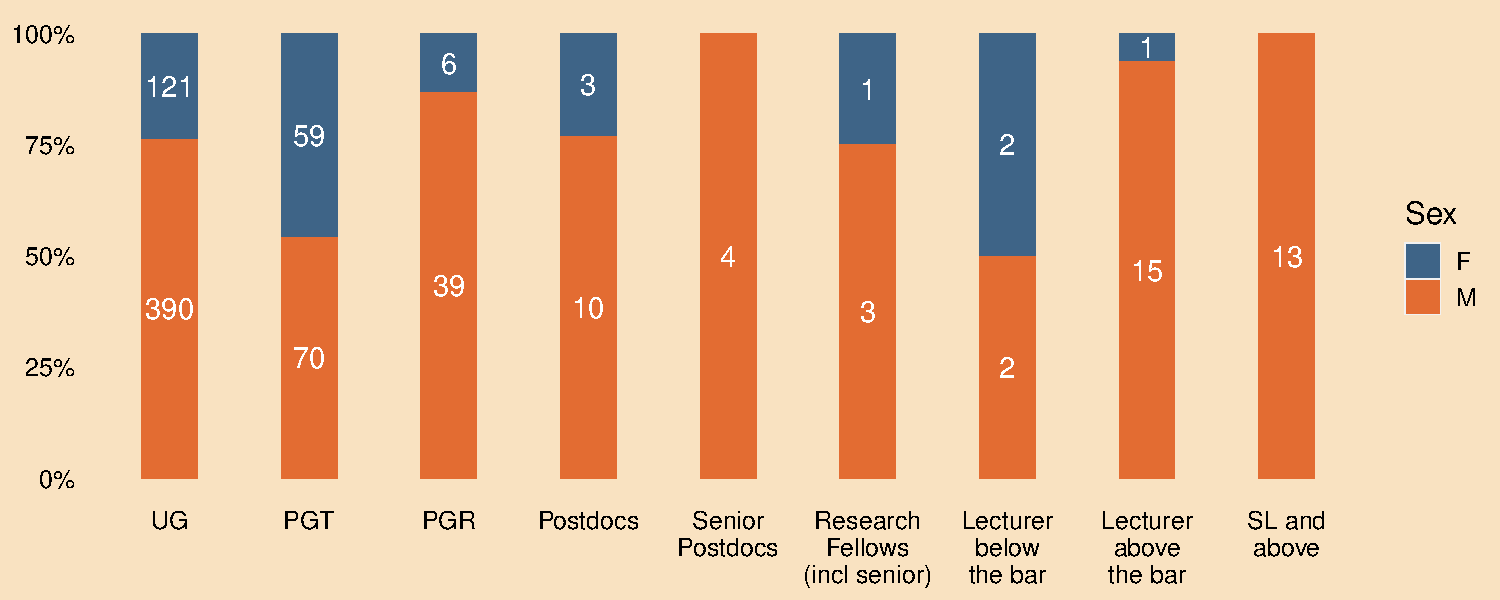
\includegraphics[width=5.5in]{fig/pipeline.pdf}
    
    \label{fig:pipeline}
\end{minipage}
}
\end{figure}

% \todo{[KJS: Insert figure "The career pipeline"; Tweak to include 
% undergraduates (24\%) and taught postgraduate (46\%) bars.
% See email of 2 Aug 2022.]}

We have included only the data for 2020 here. 
The tapering proportion of females from undergraduates to lecturers to senior 
academics is a global phenomenon in computer science, but the complete
lack of females in senior grades at UCC is an outlier even within our traditional
male-dominated discipline. As noted above, for TCD the percentage has
consistently been above 20\%.

The greatest choke points appear to be:
\begin{enumerate}[noitemsep]
    \item From undergraduate to PhD students
    \item From research roles to academic ones
    \item From lecturer to senior lecturer and beyond
\end{enumerate}

Relatively few CSIT graduates proceed to postgraduate studies and 
many of our postgraduate students are  recruited from overseas, in particular China and India.
Employment prospects for Irish computing graduates are buoyant and, 
unlike other STEM disciplines, further postgraduate study is not a 
prerequisite for flourishing careers in  industry. Indeed, some of our 
undergraduates with expertise in sought-after fields such as computer 
security can be tempted by the prospect of lucrative 
job offers to leave even before their (undergraduate)
graduation.

The factors deterring research students and postdocs from pursuing 
academic careers are explored further in 
Section~\ref{sec:academic}. 
Poor PhD stipends (currently at \texteuro{}18,500 p.a.) and low
pay for postdoctoral positions relative to attractive industry salaries 
is one factor: starting salaries on offer to talented 
graduates can be a multiple of the PhD stipend. 
Precarity and the uncertainties surrounding  securing academic 
positions and promotional opportunities thereafter is another. 
The current dire housing situation in Ireland deters potential 
applicants at all levels, especially those from abroad.


As noted above, CSIT has no female academics at \ac{SL}
rank or above, so the Lecturer/SL boundary represents
a significant choke point.
At UCC academics can attain a senior grade 
either through promotion or direct appointment to an advertised 
position. Promotion criteria and processes at UCC are 
dictated entirely 
by the University and the School has had very limited success with 
promotions over the years.
In the past twenty years there have been six academic
promotions in all (none since 2014 and no females as CSIT did not have any female academics until 2017), 
but only three from Lecturer to 
SL (most recently in 2008).
In the most recent round (2018-2019), only two 
Lecturers from CSIT applied for promotion to SL, and neither was successful.  
If promotions are to contribute to improving gender balance at senior 
levels, the school will need to analyse historical barriers to promotion
and plan to more  proactively support colleagues, particularly
females, in navigating UCC's promotion scheme successfully. 

Section~\ref{sec:academic} explores staff experiences
and perception with recruitment and  promotions and presents a suite of actions to help improve the gender balance over time.




\subsection{Provide data for professional, managerial and support staff by gender and grade. Analyse representation, benchmarking where possible.}


% \khcomment{TCD website may allow benchmarking for sysadmin staff}

Table~\ref{tab:pmsstaff} gives an overview of the numbers of professional,
managerial and support staff. For historical reasons, UCC classifies
IT staff in the school's \ac{CSSS} as 
``administrative'' rather than ``technical.''


\input{tables2/tab_pms_staff}

Among those in administrative roles in the school's office, 
females predominate, while the School's core IT support staff 
are exclusively male. A similar pattern emerges among the 
administrative and IT roles among the research support staff.
This over-representation of females in administrative roles mirrors
the situation within the University.
Section~\ref{sec:pms} explores this issue in greater depth 
and presents actions to move the school on a more gender-balanced
trajectory for PMS staff.

By way of comparison, TCD's webpage currently lists 24 administrative 
staff (21 female, 3 male), nine IT support staff (three female, six
male) and six staff classified as technicians (all male).

\subsection{Provide data on staff on fixed-term contracts, contracts of indefinite duration/permanent contracts, and hourly-paid contracts by gender and staff category. Outline instances where fixed-term and hourly-paid contract types are used. This should include comment on:}
\instr{
\begin{itemize}
    \item whether or not numbers of fixed-term/hourly-paid contracts are representative of a typical year; 
    \item the rationale for the use of short-term contracts;
    \item the extent to which hourly-paid staff contribute to the teaching of core modules and/or services.
\end{itemize}
}

\subsubsection{Representativeness of fixed-term/hourly paid contracts}

Table~\ref{tab:fthpstaff} summarises academic staff on fixed-term
contracts or hourly paid for 2020. These numbers vary from year to year, but these are fairly typical.
Table~\ref{tab:acresstaff} lists all research staff, all of whom have fixed-term contracts due to the limited lifespan of projects, and thus are not listed here. 
%Research staff are omitted as all are on fixed-term contracts as noted earlier. 
There were 
no fixed-term or hourly-paid administrative staff. 

\begin{tabbox}[11cm]{!th}

\caption{CSIT staff on fixed-term contracts and hourly-paid lecturing staff 
(2020)}
\label{tab:fthpstaff}
\footnotesize 

      
\begin{tabular}{p{4cm}
                C{1cm}
                C{1cm}
                C{1cm}
                p{0.7cm}
                C{1cm}
                C{1cm}
                C{1cm}}
\toprule 
%\multicolumn{7}{c}{\bfseries Academics and Researchers (2020)}\\ \hline
  & \multicolumn{3}{c}{Fixed-Term} && \multicolumn{3}{c}{Hourly-Paid}\\
  \cmidrule{2-4}\cmidrule{6-8}
  Position & {F} & {M} & \%F && {F} & {M} & \%F\\
  \midrule 

  Lecturer (above bar)&- & 1 & - && - &- &-\\
  Lecturer (below bar)& 1&2 & 33\% && - &- &-\\
\bottomrule 
\end{tabular}

\end{tabbox}


% \todo{
% Precise numbers vary somewhat from year to year, but these
% are fairly typical. Research staff numbers ebb and flow according
% to the funded lifespan of the various research projects and the 
% number of fixed-term academic staff also varies as needed to
% fill any short-term staffing gaps as explained below.
% }

\subsubsection{Rationale for using short-term contracts}
\label{rationalecontracts}

Short term academic contracts (typically one year) are used mainly 
to cover temporary vacancies in permanent posts arising from
maternity cover, retirements, etc. until the post can be filled on
a permanent basis. The University often sanctions posts tied
to new programmes initially on a fixed-term basis to be 
converted into permanent posts if the increased student
numbers flowing from that programme prove sustainable.

The classification of academic posts as either permanent/\ac{CID} or
fixed-term is dictated by the University, but the school advocates
to minimise the number of colleagues on fixed-term contracts.
% DT: Fixed terms 2020: LAB={RM}; LBB = {LM. JQ}
For example, two of the fixed-term lecturers shown in 
Table~\ref{tab:fthpstaff} have subsequently received 
permanent positions (both female).


Research activity is wholly dependent on the flow of research 
funding which is necessarily impermanent and so all researchers 
are on fixed-term contracts. A number of those in research 
administration or research IT support roles have 
permanent/\ac{CID} positions. These are typically admin staff
with a permanent/\ac{CID} position who are appointed to a 
higher-grade role funded by research funds.

\subsubsection{Contribution of hourly-paid staff to teaching and services}

The bulk of hourly paid staff are undergraduate or postgraduate students
employed on a part-time basis to support the school's teaching activities. 
Roles such as demonstrators for our laboratory teaching or tutors for
undergraduate modules are generally filled this way. The amount of work
provided on an hourly-paid basis varies from year to year depending
on institutional/school funding constraints and the general volume
of teaching requiring such support. In 2019-20, for example,
we had 65 hourly paid staff, 11 female and 54 male, i.e., about 
17\% female, which is somewhat below the percentage of female  
undergraduate and taught postgraduate  students.

Each year, two or three modules (each 5 ECTS)
%than 10 to 15 credits of the school's annual total of around
% \todo{XXX} credits, is 
are covered on an hourly-paid basis. This typically arises
to cover a handful of modules that either would not justify a 
full-time fixed-term contract or disparate modules requiring 
expertise that that would be difficult for one individual to 
cover. These hourly-paid lecturers are typically 
postdocs seeking some teaching experience who have the required 
expertise to teach the module(s).

% \khcomment{Clarify school's total teaching load (in credits).
% }

% Dummy newcommand to mask errors due to old deleted actions.
\newcommand{\actdeptsurvey}{Deleted}
\newcommand{\actdeptmarketing}{Amended}
\newcommand{\actdeptrolemodels}{Amended}
\newcommand{\actdeptfunds}{Deleted}
\newcommand{\actdeptcareerchoice}{Amended}
\newcommand{\actdeptpromisingfemale}{Amended}
\newcommand{\actdeptringfence}{Deleted}
\newcommand{\actdepthighlight}{Amended}
\newcommand{\actdeptseminar}{Deleted}
\newcommand{\actdeptinternships}{Amended}



